7\section{Logic and the Language of Proofs}\label{sec:logic}

In order to read and construct proofs, we need to start with the language in which they are written: \emph{logic.} Logic is to mathematics what grammar is to English. Section \ref{sec:prop} will not look particularly mathematical, but we'll quickly get to work in Section \ref{sec:proof} using logic in a mathematical context.

\subsection{Propositions}\label{sec:prop}

\begin{defn}
A \textbf{proposition} or \textbf{statement} is an expression that is either true or false.
\end{defn}

\begin{examples}\itemsep0pt
	\item $17-24=7$.
	\item $39^2$ is an odd integer.
	\item The moon is made of cheese.
	\item Every cloud has a silver lining.
	\item God exists.
\end{examples}

\noindent In order to make sense, these propositions require a clear \emph{definition} of every concept they contain. There are many concepts of God in many cultures, but once it is decided \emph{which} we are talking about, it is clear that They either exist or do not. This example illustrates that a statement need not be indisputably true or false, or even determinable, in order to qualify as a proposition. Mostly when people argue over propositions and statements, what they are really disagreeing about are definitions!\\
Note that any expression that is neither true nor false is not a proposition. \emph{January 1$^{\text{st}}$} is not a proposition, neither is \emph{Green.}

\subsubsection*{Truth Tables}

One often has to deal with abstract propositions; those where you do not know the truth or falsity, or indeed when you don't explicitly know the proposition! In such cases it can be convenient to represent the combinations of propositions in a tabular format. For instance, if we have two propositions ($P$ and $Q$), or even three ($P,Q$ and $R$) then all possible combinations of truth $T$ and falsehood $F$ are represented in the following tables:
\[\begin{array}{cc}
P & Q\\\hline
T & T\\
T & F\\
F & T\\
F & F\\
&\\&\\&\\&
\end{array}
\qquad\qquad\qquad
\begin{array}{ccc}
P & Q & R\\\hline
T & T & T\\
T & T & F\\
T & F & T\\
T & F & F\\
F & T & T\\
F & T & F\\
F & F & T\\
F & F & F
\end{array}\]
The mathematician in you should be looking for patterns and asking: how many rows would a truth table corresponding to $n$ propositions have, and can I \emph{prove} my assertion? Right now it is hard to prove that the answer is $2^n$: induction (Chapter \ref{sec:ind}) makes this very easy.

\subsubsection*{Connecting Propositions: Conjunction, Disjunction and Negation}

We now \emph{define} how to combine propositions in natural ways, modeled on the words \emph{and, or} and \emph{not.}

\begin{defn}
Let $P$ and $Q$ be propositions. The \textbf{conjunction} (AND, $\wedge$) of $P$ and $Q$, the \textbf{disjunction} (OR, $\vee$) of $P$ and $Q$, and the \textbf{negation} (NOT, $\neg$, $\sim$, $\cl{\phantom{P}}$) of $P$ are defined by the following truth tables,
\[\begin{array}{cc|c}
P & Q & P\wedge Q\\\hline
T & T & T\\
T & F & F\\
F & T & F\\
F & F & F
\end{array}\qquad\qquad
\begin{array}{cc|c}
P & Q & P\vee Q\\\hline
T & T & T\\
T & F & T\\
F & T & T\\
F & F & F
\end{array}\qquad\qquad
\begin{array}[b]{c|c}
P & \neg P\\\hline
T & F\\
F & T
\end{array}\]
\end{defn}

\noindent It is usually better to use \emph{and, or} and \emph{not} rather than \emph{conjunction, disjunction} and \emph{negation}: the latter may make you sound educated, but at the risk of being misunderstood!

\begin{example}
Let $P,Q$ and $R$ be the following propositions:
\begin{itemize}
\item[]\itemstart{$P$.} Irvine is a city in California.
\item[]\itemstart{$Q$.} Irvine is a town in Ayrshire, Scotland.
\item[]\itemstart{$R$.} Irvine has seven letters.
\end{itemize}
Clearly $P$ is true while $R$ is false. If you happen to know someone from Scotland, you might know that $Q$ is true.\footnote{The second syllable is pronounced like the i in bin or win. Indeed the first Californian antecedent of the Irvine family which gave its name to UCI was an Ulster-Scotsman named James Irvine (1827--1886). Probably the family name was originally pronounced in the Scottish manner.} We can now compute the following (increasingly grotesque) combinations\ldots
\[\def\arraystretch{1.3}
\begin{array}{c|c|c|c|c|c|c}
P\wedge Q&P\vee Q&P\wedge R&\neg R&(\neg R)\wedge P&\neg(R\vee P)&(\neg P)\vee [((\neg R)\vee P)\wedge Q] \\\hline
T & T & F & T & T & F & T
\end{array}\]
\end{example}

\noindent How did we establish these facts? Some  are quick,  and can be done in your head. Consider, for instance, the statement  $(\neg R)\wedge P$. Because $R$ is false, $\neg R$ is true. Thus $(\neg R)\wedge P$ is the conjunction of two true statements, hence it is true. Similarly, we can argue that $R\vee P$ is true (because $R$ is false and $P$ is true), so the negation $\neg(R\vee P)$ is false.

\noindent  Establishing the truth value of the final proposition $(\neg P)\vee [((\neg R)\vee P) \wedge Q]$ requires more work. You may want to set up a truth table with several auxiliary columns to help you compute: 
\[\def\arraystretch{1.3}
\begin{array}{c|c|c|c|c|c|c|c}
P & Q & R & \neg P & \neg R & (\neg R) \vee P & ((\neg R)\vee P) \wedge Q &  (\neg P) \vee [ ((\neg R)\vee P) \wedge Q] \\\hline
 T & T & F & F            & T         & T                        & T                                               & T
 \end{array}\]
The importance of parentheses in a logical expressions cannot be stressed enough. For example, try building the truth table for the propositions $P\vee(Q\wedge R)$ and $(P\vee Q)\wedge R$. Are they the same?%\pagebreak[4]


\subsubsection*{Conditional and Biconditional Connectives}

In order to logically set up proofs, we need to see how propositions can lead one to another.

\begin{defn}\label{defn:implies}
The \textbf{conditional} ($\implies$) and \textbf{biconditional} ($\iff$) \emph{connectives} have the truth tables
\[\begin{array}{cc|c}
P & Q & P\implies Q\\\hline
T & T & T\\
T & F & F\\
F & T & T\\
F & F & T
\end{array}\qquad\qquad\qquad
\begin{array}{cc|c}
P & Q & P\iff Q\\\hline
T & T & T\\
T & F & F\\
F & T & F\\
F & F & T
\end{array}\]
For the proposition $\timplies P{Q,}$ we call $P$ the \textbf{hypothesis} and $Q$ the \textbf{conclusion}.
\end{defn}

\noindent Observe that the expressions $\timplies PQ$ and $\ P\iff Q\ $ are themselves \emph{propositions}: they are sentences which are either true or false!

\subsubsection*{Synonyms}

$\implies$ and $\iff$ can be read in many different ways:
\begin{center}
\begin{tabular}{c|c}
$P\implies Q$ & $P\iff Q$\\\hline
$P$ implies $Q$ & $P$ if and only if $Q$\\
$Q$ if $P$ & $P$ iff $Q$\\
% $P$ only if $Q$ & $P$ is necessary and sufficient for $Q$\\
% $P$ is sufficient for $Q$ & \\
$P$ only if $Q$ & $P$ and $Q$ are equivalent\\
$P$ is sufficient for $Q$ &$P$ is necessary and sufficient for $Q$\\
$Q$ is necessary for $P$ &
\end{tabular}
\end{center}

\begin{example}
The following propositions all mean exactly the same thing:
\begin{itemize}
\item If you are born in Rome, then you are Italian. 
\item You are Italian if you are born in Rome. 
\item You are born in Rome only if you are Italian. 
\item Being born in Rome is sufficient to be Italian. 
\item Being Italian is necessary for being born in Rome. 
\end{itemize}
\end{example}


\noindent Are you comfortable with what $P$ and $Q$ are here?\\

\noindent The biconditional connective should be easy to remember: $\ P\iff Q\ $ is true precisely when $P$ and $Q$ have identical truth states. It is harder to make sense of the conditional connective. One way of thinking about it is to consider what it means for an implication to be \emph{false.} If $P\implies Q$ is false, it is impossible to create a logical argument which assumes $P$ and concludes $Q$. The second row of $\timplies PQ$ encapsulates the fact that it should be impossible for truth ever to logically imply falsehood. 

%\begin{nopgbreak}
\begin{aside}
\noindent{\bf Why is $F\implies T$ considered \emph{true?}}

This is the most immediately confusing part of the truth table for the conditional connective. One way that may help to remember this is to think of the implication $P \implies Q$ as making a promise. For example, suppose your teacher says: ``if the class earns a B average on the midterm exam, then I will buy donuts for the class.'' Under what circumstances will your teacher have lied to you? Only in the case that it is true that the class earned a B average, but the teacher failed to provide donuts for the class. 

Here is a mathematical example, written with an English translation at the side.
\begin{align*}
7=3\implies\ &0\cdot 7=0\cdot 3\tag*{(If $7=3$, then 0 times 7 equals 0 times 3)}\\
\implies\ &0=0\tag*{(then 0 equals 0)}
\end{align*}
Thus $7=3\implies 0=0$. Logically speaking this is a perfectly correct argument, thus the \emph{implication} is true. The argument makes us uncomfortable because $7=3$ is clearly false.



% If you want to understand connectives more deeply than this, then take a logic or philosophy course! For example, although neither statement makes the least bit of sense in English;
% \begin{center}
% ``17 is odd $\implies$ Mexico is in China'' is \emph{false,}\\ whilst\\
% ``17 is even $\implies$ Mexico is in China'' is \emph{true.}
% \end{center}
% Such bizarre constructions are happily beyond the consideration of this course!
\end{aside}
%\end{nopgbreak}


\subsubsection*{Theorems and Direct Proofs}

Truth tables and connectives are very abstract. To apply them to mathematics we need the following basic notions of theorem and proof.

\begin{defn}
A \textbf{theorem} is a justified assertion that some statement of the form $\timplies PQ$ is true.\\
A \textbf{proof} is an argument that justifies the truth of a theorem.
\end{defn}

\noindent Think back to the truth table for $\timplies PQ$ in Definition \ref{defn:implies}. Suppose that the hypothesis $P$ is true and that $\timplies PQ$ is true: that is, $\timplies PQ$ is a \emph{theorem.} We must be in the \emph{first row} of the truth table, and so the conclusion $Q$ is also true. This is how we think about proving basic theorems. In a \emph{direct proof} we start by assuming the hypothesis ($P$) is true and make a logical argument ($P\implies Q$) which asserts that the conclusion ($Q$) is true. As such, it often convenient to rewrite the statement of a theorem as an implication of the form $\timplies P{Q.}$ Here is a very simple theorem which we prove directly. 

\begin{thm}
The product of two odd integers is odd.
\end{thm}

\noindent The first thing to do is to write the theorem in terms of propositions and connectives: that is, in the form $P\implies Q$.
\begin{itemize}
  \item $P$ is `$x$ and $y$ are odd integers.' This is our assumption, the hypothesis.
  \item $Q$ is `The product of $x$ and $y$ is odd.' This is what we want to show, the conclusion.
  \item Showing that $\timplies PQ$ is true, that (the truth of) $P$ implies (the truth of) $Q$ requires an argument. This is the \emph{proof.}
\end{itemize}

\begin{proof}
Let $x$ and $y$ be \emph{any} two odd integers. We want to show that product $x\cdot y$ is an odd integer. \\
By definition, an integer is odd if it can be written in the form $2k+1$ for \emph{some} integer $k$. Thus there must be integers $n$, $m$ such that $x=2n+1$ and $y=2m+1$. We compute:
\[x\cdot y=(2n+1)(2m+1)=4mn+2n+2m+1=2(2mn+n+m)+1.\]
Because $2mn+n+m$ is an integer, this shows that $x\cdot y$ is an odd integer.
\end{proof}

\noindent It is common to place a symbol (in this case \smash{\raisebox{7pt}{$\qedsymbol$}}) at the end of a proof to tell the reader that your argument is complete. Traditionally the letters Q.E.D. (from the Latin \emph{quod erat demonstrandum,} literally `which is what had to be demonstrated') were used, but this has gone out of style.You may also feel that you want to write more, or less than the above. This is a difficult thing to judge. What do you feel is a convincing argument? Test your argument on your classmates. The appropriate level of detail will depend on your readership: a middle school student will need more detail than a graduate student! At the moment, the best guide is to write for someone with the same mathematical sophistication as yourself. If, in three weeks' time, you can return to what you've written and understand it, then it's probably good!


\subsubsection*{The Converse and Contrapositive}

The following constructions are used continually in mathematics: it is vitally important to know the difference between them.

\begin{defn}\label{defn:contra}
The \textbf{converse} of an implication $\timplies PQ$ is the reversed implication $\timplies Q{P.}$\\
The \textbf{contrapositive} of $\timplies PQ$ is $\timplies{\neg Q}{\neg P.}$
\end{defn}

\noindent In general, we cannot say anything about the truth value of the converse of a true implication. The contrapositive of a true implication is, however, \emph{always} true. Actually, even more is true, an implication and its contrapositive always have the same truth value. This is a common enough phenomenon that we give it its own name.

\begin{defn}\label{defn:logequiv}
We say two propositions are \textbf{logically equivalent} if they have the same truth table.
\end{defn}

\noindent This definition is a bit vague (what does having the same truth table mean?) We could give a more rigorous definition, but instead hope that the following examples will make the definition clear.

\begin{example}
We prove that the expressions $(P\implies Q) \wedge (Q\implies P)$ and $\ P\iff Q\ $ are logically equivalent by computing their truth tables:
\[
\begin{array}{cc|c|c|c}
P & Q & P\implies Q & Q \implies P & (P \implies Q) \land (Q \implies P) \\
\hline
T & T & T & T & \mathbf T \\
T & F & F & T & \mathbf F \\
F & T & T & F & \mathbf F \\
F & F & T & T & \mathbf T
\end{array} \qquad \begin{array}{cc|c}
P & Q & P \iff Q \\
\hline
T & T & \mathbf T \\
T & F & \mathbf F \\
F & T & \mathbf F \\
F & F & \mathbf T 
\end{array}
\]
Notice that the bolded columns are the same in each table.
\end{example}

\noindent Note that when comparing truth tables, one should make sure the inputs (e.g. the columns for $P$ and $Q$ in the above example) are in the same order in both tables.

\begin{thm}\label{thm:contrapos}
The contrapositive of an implication is logically equivalent the original implication.
\end{thm}

\begin{proof}
Simply use our definitions of negation and implication to compute the truth table:
\begin{gather*}
\begin{array}{cc|c||cc|c}
P & Q & P\implies Q & \neg Q & \neg P & \neg Q\implies\neg P\\\hline
T & T & \mathbf T & F & F & \mathbf T\\
T & F & \mathbf F & T & F & \mathbf F\\
F & T & \mathbf T & F & T & \mathbf T\\
F & F & \mathbf T & T & T & \mathbf T
\end{array}
\end{gather*}
Since the truth states in the third and sixth columns (in bold) are identical, we see that $\timplies PQ$ and its contrapositive $\timplies{\neg Q}{\neg P}$ are logically equivalent.
\end{proof}

\begin{example}
Let $P$ and $Q$ be the following statements:
\begin{itemize}\setlength{\itemsep}{0pt}
  \item[]\itemstart{$P$.} Claudia is holding a peach.
  \item[]\itemstart{$Q$.} Claudia is holding a piece of fruit.
\end{itemize}
The implication $P\implies Q$ is true, since all peaches are fruit. As a sentence, we have:
\begin{itemize}\setlength{\itemsep}{0pt}
  \item[]If Claudia is holding a peach, then Claudia is holding a piece of fruit.
\end{itemize}
The \emph{converse} of $P\implies Q$ is the sentence:
\begin{itemize}\setlength{\itemsep}{0pt}
  \item[]If Claudia is holding a piece of fruit, then Claudia is holding a peach.
\end{itemize}
This is palpably false: Claudia could be holding an apple!\\\pagebreak[2]

\noindent The \emph{contrapositive} of $P\implies Q$ is the following sentence:
\begin{itemize}\setlength{\itemsep}{0pt}
  \item[]If Claudia is \emph{not} holding any fruit, then she is \emph{not} holding a peach.
\end{itemize}
This is clearly true.
\end{example}



\subsubsection*{Proof by Contrapositive}

The fact that $\timplies PQ$ and $\timplies{\neg Q}{\neg P}$ are logically equivalent allows us, when convenient, to prove $\timplies PQ$ by instead proving its contrapositive. As an example, consider another basic theorem.

\begin{thm}
Let $x$ and $y$ be integers. If $x+y$ is odd, then exactly one of $x$ or $y$ is odd.
\end{thm}

\noindent The theorem is an implication of the form $\timplies PQ$ where
\begin{itemize}\setlength{\itemsep}{0pt}
  \item[]\itemstart{$P$.} The sum $x+y$ of integers $x$ and $y$ is odd.
  \item[]\itemstart{$Q$.} Exactly one of $x$ or $y$ is odd.
\end{itemize}

\noindent A direct proof would require that we assume $P$ to be true and logically deduce the truth of $Q$. For instance we might start our argument with:
\[\text{Suppose that $x+y=2n+1$ for some integer $n$}\]
The problem is that this doesn't really tell us anything about $x$ and $y$, which we need to think about in order to demonstrate the truth of $Q$. Instead we consider the negations of our propositions:
\begin{itemize}\setlength{\itemsep}{0pt}
  \item[]\itemstart{$\neg Q$.}\quad $x$ and $y$ are both even or both odd \ (they have the same parity).
  \item[]\itemstart{$\neg P$.}\quad The sum $x+y$ of integers $x$ and $y$ is even.
\end{itemize}
Since $\timplies PQ$ is logically equivalent to the seemingly simpler contrapositive $\timplies{(\neg Q)}{(\neg P),}$ we choose to prove the latter. This is, by Theorem \ref{thm:contrapos}, equivalent to proving the original implication.

\begin{proof}
Assume that $x$ and $y$ have the same parity. There are two cases: $x$ and $y$ are both even, or both odd.
\begin{description}\setlength{\itemsep}{0pt}
  \item[Case 1:] Let $x=2m$ and $y=2n$ be even. Then $x+y=2(m+n)$ is even.
  \item[Case 2:] Let $x=2m+1$ and $y=2n+1$ be odd. Then $x+y=2(m+n+1)$ is even.
\end{description}
In both cases $x+y$ is even, and the result is proved.
\end{proof}

 
\subsubsection*{De Morgan's Laws}

In order to perform proofs by contrapositive (and later by contradiction) it is necessary to compute the negations of propositions. The most helpful results in this regard are attributable to Augustus de Morgan, a very famous 19th century logician.


\begin{thm}[de Morgan's laws]\label{thm:demorgan}
Let $P$ and $Q$ be any propositions. Then:
\begin{enumerate}\setlength{\itemsep}{0pt}
  \item $\neg(P\wedge Q)$ is logically equivalent to  $\neg P\vee\neg Q$.
  \item $\neg(P\vee Q)$ is logically equivalent to $\neg P\wedge\neg Q$.
\end{enumerate}
\end{thm}

%\noindent The first law says that the negation of $P\wedge Q$ is logically equivalent to $\neg P\vee\neg Q$: that is, the two expressions have the \emph{same truth table.} 

\noindent Here is a proof of the first law. Try the second on your own.

\begin{proof}
$\begin{array}[t]{cc|cc|ccc}
P & Q & P\wedge Q & \neg(P\wedge Q) & \neg P & \neg Q & \neg P\vee\neg Q\\\hline
T & T & T & \mathbf F & F & F & \mathbf F\\
T & F & F & \mathbf T & F & T & \mathbf T\\
F & T & F & \mathbf T & T & F & \mathbf T\\
F & F & F & \mathbf T & T & T & \mathbf T
\end{array}$

Simply observe that the fourth and seventh columns are identical.
\end{proof}

\noindent It is worth pausing to observe how similar the two laws are, and how concise. There is some beauty here. With a written example the laws are much easier to comprehend. 

\begin{example}
(Of the first law) Suppose that of a morning you can choose (or not) to ride the subway to work, and you can choose (or not) to have a cup of coffee. Consider the following sentence:
\begin{itemize}\setlength{\itemsep}{0pt}
  \item[] I rode the subway \emph{and} I had coffee.
\end{itemize}
What would it mean for this sentence to be \emph{false?} Any sentence which asserts the falsehood of the above is a suitable \emph{negation.} For example:
\begin{itemize}\setlength{\itemsep}{0pt}
  \item[] I \emph{didn't} ride the subway \emph{or} I \emph{didn't} have coffee.
\end{itemize}
Note that the mathematical use of \emph{or} includes the possibility that you neither rode the subway nor had coffee.
\end{example}

\noindent You will see de Morgan's laws again when we encounter sets.

\begin{aside}
\noindent{\bf Think about the meaning!}

In the previous example we saw how negation switches \emph{and} to \emph{or.} This is true only when \emph{and} denotes a conjunction between two propositions. Before applying De Morgan's laws, think about the \emph{meaning} of the sentence. For example, the negation of
\begin{itemize}\setlength{\itemsep}{0pt}
  \item[] Mark and Mary have the same height.
\end{itemize}
is the proposition:
\begin{itemize}\setlength{\itemsep}{0pt}
  \item[] Mark and Mary do not have the same height.
\end{itemize}
If you blindly appeal to De Morgan's laws you might end up with the following piece of nonsense:
\begin{itemize}\setlength{\itemsep}{0pt}
  \item[] Mark \emph{or} Mary do not have the same height.
\end{itemize}
Logical rules are wonderfully concise, but very easy to misuse. Always think about the meaning of a sentence and you shouldn't go wrong.
\end{aside}
 
\subsubsection*{Negating Conditionals}

You will often want to understand the negation of a statement. In particular, it is important to understand the negation of a conditional $\timplies P{Q.}$ Is it enough to say `$P$ doesn't imply $Q$'? And what could this mean? To answer the question you can use truth tables, or just think.

\noindent Here is the truth table for $\timplies PQ$ and its negation: recall that negation simply swaps $T$ and $F$.
\[\begin{array}{cc|c|c}
P & Q & P\implies Q & \neg(P\implies Q)\\\hline
T & T & T & F\\
T & F & F & T\\
F & T & T & F\\
F & F & T & F
\end{array}\]
The only time there is a $T$ in the final column is when \emph{both} $P$ is true \emph{and} $Q$ is false. We have therefore proved the following:

\begin{thm}\label{thm:negconditional}
$\neg(P\implies Q)$ is logically equivalent to $P\wedge\neg Q$ \ (read `$P$ and not $Q$').
\end{thm}

\noindent Now \emph{think} in words rather than calculate. What is the negation of the following implication?
\begin{itemize}\setlength{\itemsep}{0pt}
  \item[] It's the morning therefore I'll have coffee.
\end{itemize}
Hopefully it is clear that the negation is:
\begin{itemize}\setlength{\itemsep}{0pt}
  \item[] It's the morning \emph{and} I \emph{won't} have coffee.
\end{itemize}

\noindent The implication \emph{`therefore'} has disappeared and the expression \emph{`and won't'} is in its place.\\

\noindent{\bf Warning!} The negation of $\timplies PQ$ is \emph{not a conditional.} In particular it is \emph{neither} of the following:
\begin{itemize}\setlength{\itemsep}{0pt}
  \item[] The converse, $Q\implies P$.
  \item[] The contrapositive of the converse, $\neg P\implies\neg Q$. 
\end{itemize}
If you are unsure about this, write down the truth tables and compare.\goodbreak

\begin{example}
Let $x$ be an integer. What is the negation of the following sentence?
\begin{itemize}\setlength{\itemsep}{0pt}
  \item[] If $x$ is even, then $x^2$ is even.
\end{itemize}
Written in terms of propositions, we wish to negate $\timplies PQ$, where $P$ and $Q$ are:
\begin{itemize}\setlength{\itemsep}{0pt}
  \item[]\itemstart{$P.$} $x$ is even.
  \item[]\itemstart{$Q.$} $x^2$ is even.
\end{itemize}
The negation of $P\implies Q$ is $P\wedge\neg Q$, namely:
\begin{itemize}\setlength{\itemsep}{0pt}
  \item[] $x$ is even and $x^2$ is odd.
\end{itemize}
This is very different to $\timplies{\neg P}{\neg Q}$ (if $x$ is odd then $x^2$ is odd).\\[5pt]
Keep yourself straight by thinking about the meaning of these sentences. It should be obvious that `$x$ even $\implies x^2$ even' is true. It negation should therefore be \emph{false.} The fact that it is false should make reading the negation feel a little uncomfortable.
\end{example}




\subsubsection*{Tautologies and Contradictions}

We finish this section with two related concepts that are helpful for understanding proofs.

\begin{defn}
A \textbf{tautology} is a logical expression that is always true, regardless of what the component statements might be.\\
A \textbf{contradiction} is a logical expression that is always false.
\end{defn}

\noindent The easiest way to detect these is simply to construct a truth table. We remark that two propositions $\varphi$ and $\psi$ are logically equivalent if and only if $\varphi \iff \psi$ is a tautology.

\begin{examples}
	\item $P\wedge(\neg P)$ is a very simple contradiction:
	\[\begin{array}{cc|c}
	P & \neg P & P\wedge(\neg P)\\\hline
	T & F & F\\
	F & T & F
	\end{array}\]
	Whatever the proposition $P$ is, it cannot be true at the same time as its negation.
	\item $(P\wedge(P\implies Q))\implies Q$ \ is a tautology. This is essentially how we understand a direct proof: if $P$ is true and we have a correct argument $P\implies Q$, then $Q$ must also be true.
	\[\begin{array}{cc|cc|c}
	P & Q & P\implies Q & P\wedge(P\implies Q) & (P\wedge(P\implies Q))\implies Q\\\hline
	T & T & T & T& T\\
	T & F & F & F& T\\
	F & T & T & F& T\\
	F & F & T & F& T
	\end{array}\]
	%\item $(P\wedge \neg Q\implies F)\iff (P\implies Q)$ is a tautology. This tautology is the basis for \emph{proof by contradiction,} as we'll see in the next section. The expression $P\wedge \neg Q\implies F$ can be thought of as saying that $P\wedge\neg Q$ implies a contradiction.
\end{examples}\goodbreak

\begin{aside}
\noindent{\bf Algebraic Logic}

One can study logic in a more algebraic manner. De Morgan's Laws are algebraic. Here are a few of the other basic laws of logic.
\begin{align*}\label{aside:logicalalg}\hypertarget{aside:logicalalglnk}{}
&\text{Law of Double Negation}: \\
&\neg(\neg P) \quad \text{is logically equivalent to} \quad P \\
&\text{Commutative laws}: \\
&P\wedge Q \quad \text{is logically equivalent to} \quad Q\wedge P \\
&P\vee Q \quad \text{is logically equivalent to} \quad Q\vee P\\
&\text{Associative laws}: \\
&(P\wedge Q)\wedge R \quad \text{is logically equivalent to} \quad P\wedge(Q\wedge R) \\
&(P\vee Q)\vee R \quad \text{is logically equivalent to} \quad P\vee(Q\vee R)\\
&\text{Distributive laws}: \\
&(P\wedge Q)\vee R \quad \text{is logically equivalent to} \quad (P\vee R)\wedge (Q\vee R) \\
&(P\vee Q)\wedge R \quad \text{is logically equivalent to} \quad (P\wedge R)\vee (Q\wedge R)
\end{align*}
You can check them all with truth tables. Using these rules, one can answer questions, such as deciding when an expression is a tautology, without laboriously creating truth tables. It is even fun! Such an approach is appropriate when you are  considering abstract propositions, say in a formal logic course. In this text our primary interest with logic lies in using it to prove theorems. When one has an explicit theorem it is important to keep the meanings of all propositions clear. By relying too much on abstract laws like the above, it is easy to lose the meaning and write nonsense! 
\end{aside}



% \paragraph{Self-test Questions} (fill in the blanks or select the correct word) 

% \begin{itemize}
%   \item A \emph{tautology} is a proposition which \underline{\phantom{is always true}\qquad\qquad}
%   \item A \emph{contradiction} is a proposition which \underline{\phantom{is always false}\qquad\qquad}
%   \item The \emph{contrapositive} of the conditional $P\implies Q$ is the conditional \underline{\phantom{$\not Q\implies\not P$}\qquad\qquad}
%   \item The \emph{converse}/\emph{contrapositive} of $P\implies Q$ is logically equivalent to $P\implies Q$.
%   \item The converse of $P\implies Q$ is always logically equivalent to $P\implies Q$.
%   \item The \emph{negation} of the conditional $P\implies Q$ is the proposition \underline{\phantom{$\not Q\implies\not P$}\qquad\qquad}
%   \item State de Morgan's laws for propositions $P$ and $Q$:
%   \begin{gather*}
%     \neg(P\vee Q)\iff\underline{\phantom{(\neg P)\wedge (\neg Q)}\qquad}\\
%     \neg(P\wedge Q)\iff\underline{\phantom{(\neg P)\vee (\neg Q)\qquad}}
%   \end{gather*}
% \end{itemize}

\subsection*{Reading Quiz}

\begin{enumerate}
  \item A \emph{tautology} is a proposition which \underline{\phantom{is always true}\qquad\qquad}
  \begin{enumerate}
      \item is false no matter what the truth value of its component propositions.
      \item is only true when all of its component propositions are true.
      \item is never false, no matter what the truth value of its component propositions.
      \item is built only using the connectives $\land, \lor$.
  \end{enumerate}
  \item A \emph{contradiction} is a proposition which \underline{\phantom{is always false}\qquad\qquad}
  \begin{enumerate}
      \item is false no matter what the truth value of its component propositions.
      \item is only true when all of its component propositions are false.
      \item is never false, no matter what the truth value of its component propositions.
      \item is built only using the connective $\neg$.
  \end{enumerate}
  \item The \emph{contrapositive} of the conditional $P\implies Q$ is the conditional \underline{\phantom{$\not Q\implies\not P$}\qquad\qquad}
  \begin{enumerate}
      \item $\neg P \implies Q$
      \item $\neg Q \implies \neg P$
      \item $Q \implies P$
      \item $P \implies \neg Q$
  \end{enumerate}
  %\item The \emph{converse}/\emph{contrapositive} of $P\implies Q$ is logically equivalent to $P\implies Q$.
  \item True or False: The \emph{converse} of $P\implies Q$ is always logically equivalent to $P\implies Q$.
  \item The \emph{negation} of the conditional ``if I study at least 25 hours per week, then I will be successful'' is the proposition \underline{\phantom{$\not Q\implies\not P$}\qquad\qquad}
  \begin{enumerate}
      \item ``I study at least 25 hours per week, but I am not successful.''
      \item ``Either I study less than 25 hours per week, or I am successful.''
      \item ``Either I study at least 25 hours per week, or I am not successful.''
      \item `If I am successful, then I will study at least 25 hours per week.''
  \end{enumerate}
  \item De Morgan's laws state that:
  \begin{gather*}
    \neg(P\vee Q) \text{ is logically equivalent to } (1) \underline{\phantom{(\neg P)\wedge (\neg Q)}\qquad}\\
    \neg(P\wedge Q) \text{ is logically equivalent to } (2) \underline{\phantom{(\neg P)\vee (\neg Q)\qquad}}
  \end{gather*}
  \begin{enumerate}
      \item (1) $\neg (P \implies Q)$, \quad (2) $(\neg P \lor \neg Q)$
      \item (1) $(\neg P \land \neg Q)$, \quad (2) $(P \lor Q)$
      \item (1) $(\neg P \land Q)$, \quad (2) $(P \lor \neg Q)$
      \item (1) $(\neg P \land \neg Q)$, \quad (2) $(\neg P \lor \neg Q)$
  \end{enumerate}
\end{enumerate}

\subsection*{Practice Problems}

\begin{enumerate}\renewcommand{\labelenumi}{\thesubsection.\theenumi} 
  \item Suppose that ``If Colin was early, then no-one was playing pool'' is a true statement.\prelistskip
		\begin{enumerate}
	  	\item What is its contrapositive of this statement? Is it true?
	  	\item What is the converse? Is it true?
	  	\item What can we conclude (if anything?) if we discover each of the following? \emph{Treat the two scenarios separately.}
			\begin{enumerate}
	  	  \item[(i)] Someone was playing pool.
	      \item[(ii)] Colin was late.
			\end{enumerate}
		\end{enumerate}
		% (From previous exercises)
		
		\href{https://youtu.be/BI_M1-OoMac}{Video Solution}
  
  \item Prove that $P \lor \neg Q$ is logically equivalent to $\neg P \implies (\neg P \land \neg Q)$.
  
  \href{https://youtu.be/NrbdGXAP6Ug}{Video Solution}
  
  \item Define the connective $\uparrow$ (called the \emph{Sheffer stroke}, or \emph{NAND}) by the following truth table:
  \[
  \begin{array}{cc|c}
P & Q & P \uparrow Q\\\hline
T & T & F\\
T & F & T\\
F & T & T\\
F & F & T
\end{array}
  \]
  \begin{enumerate}
      \item Prove $P \uparrow Q$ is logically equivalent to $\neg (P \land Q)$. 
      \item Find an expression built using only $P$ and the connective $\uparrow$ which is logically equivalent to $\neg P$.
      \item Find an expression built using only $P$, $Q$, and the connective $\uparrow$ which is logically equivalent to $P \land Q$.
  \end{enumerate}
  
  \href{https://youtu.be/bxYgvuXtcTM}{Video Solution}
  
\end{enumerate}

\subsection*{Exercises}

\begin{enumerate}\renewcommand{\labelenumi}{\thesubsection.\theenumi}  
  \item Express each of the following statements in the ``If $\dots$, then $\dots$'' form. There are many possible correct answers.\prelistskip
		\begin{enumerate}
	  	\item You must eat your dinner if you want to grow.
	  	\item Being a multiple of 12 is a sufficient condition for a number to be even.
	  	\item It is necessary for you to pass your exams in order for you to obtain a degree. 
	  	\item A triangle is equilateral only if all its sides have the same length.
		\end{enumerate}\goodbreak
	
  \item Suppose that ``$x$ is an even integer'' and ``$y$ is an irrational number'' are true statements and that ``$z\geq 3$'' is a false statement. Which of the following are true?\\
  \emph{Hint: Label each of the given statements, and think about each of the following using connectives.}\prelistskip
		\begin{enumerate}
	  	\item If $x$ is an even integer, then $z\geq 3$.
	  	\item If $z\geq 3$, then $y$ is an irrational number.
	  	\item If $z\geq 3$ or $x$ is an even integer, then $y$ is an irrational number.
	  	\item If $y$ is an irrational number and $x$ is an even integer, then $z\geq 3$.
		\end{enumerate}
	
  \item Write the negation, the converse and the contrapositive  of the following claim:\prelistskip
		\begin{enumerate}\setlength{\itemsep}{0pt}
    \item[] If $A$ and $B$ are invertible matrices, then $AB$ is a square matrix and $\det(AB) \neq 0$. 
		\end{enumerate}
  Write your answers in sentences, like the original.

  \item Orange County has two competing transport plans under consideration: widening the 405 freeway and constructing light rail down its median. A local politician is asked, ``Would you like to see the 405 widened or would you like to see light rail constructed?'' The politician wants to sound positive, but to avoid being tied to one project. What is their response?\\
  (\emph{Hint: Think about how the word `OR' is used in logic\ldots})
  
  \item Consider the proposition $P$ given below: 
  	\begin{center}
  		If the integer $m$ is greater than 3, the integer $2m$ is not prime.
  	\end{center}
  \begin{enumerate}
    \item Rewrite $P$ using the word `necessary.'
 \item Rewrite $P$ using the word  `sufficient.'
 \item Write the negation, the converse and the contrapositive of $P$. 
  \end{enumerate}
   Write your answers in sentences, like the originals.

   
  \item Let $A$ be a square matrix. 
  Consider the proposition $Q$ given below: 
  	\begin{center}
  		For $A$ to be invertible, it is necessary and sufficient that $A$ is non-singular.
  	\end{center}
   \begin{enumerate}
    \item Rewrite $Q$ as a biconditional. 
  	\item Write the negation of $Q$. (Hint: Your answer should be the disjunction of two sentences.)
   
  \end{enumerate} 
  
  \item Let $m$ and $n$ be two integers. Consider the statement:
  \[
        m \text{ and } n \text{ are not both even}.
  \]
  \begin{enumerate}
      \item Your friend writes this statement as 
      \[
         m \land n \text{ are not both even}.
      \]
      What are some issues with what your friend wrote, if any?
      \item Then your friend claims that the negation of this statement is
      \[
         m \text{ or } n \text{ is odd}.
      \]
      Is this the correct negation? If not, what is the correct negation?
  \end{enumerate}
  
  \item Construct the truth tables for the propositions $P\vee(Q\wedge R)$ and $(P\vee Q)\wedge R$. Are they the same?
  
  \item Complete the truth table for the following proposition.
  \[
  \begin{array}{ccc|c|c|c}
	P & Q & R & P\implies Q & (P\implies Q) \land \neg R & ((P\implies Q) \land \neg R)\implies P\\\hline
	T & T & T & \phantom{T} & \phantom{F} & \phantom{T}\\
	T & T & F & \phantom{T} & \phantom{T} & \phantom{T}\\
	T & F & T & \phantom{F} & \phantom{F} & \phantom{T}\\
	T & F & F & \phantom{F} & \phantom{F} & \phantom{T}\\
	F & T & T & \phantom{T} & \phantom{F} & \phantom{T}\\
	F & T & F & \phantom{T} & \phantom{T} & \phantom{F}\\
	F & F & T & \phantom{T} & \phantom{F} & \phantom{T}\\
	F & F & F & \phantom{T} & \phantom{T} & \phantom{F}
	\end{array}
	\]
  
  \item\label{ex:demorganimplies} Apply de Morgan's laws to the result of Theorem \ref{thm:negconditional}  to prove that $\timplies PQ$ is logically equivalent to $\neg P\vee Q$. Do not use truth tables for this exercise.
  
  \item Prove the law of \emph{double negation}, i.e., that
  \[
    \neg(\neg P) \text{ is logically equivalent to } P.
  \]
  
  \item Prove that 
  \begin{enumerate}
      \item $(P \lor P)$ is logically equivalent to $P$
      \item $(P \land P)$ is logically equivalent to $P$
  \end{enumerate} 
  This is known as \emph{idempotence} for $\lor$ and $\land$, respectively.
  
  \item Prove that 
  \begin{enumerate}
      \item $P \lor (P \land Q)$ is logically equivalent to $P$
      \item $P \land (P \lor Q)$ is logically equivalent to $P$
  \end{enumerate} 
  These are known as the \emph{absorption laws}.
  
  \item Prove or disprove: $\neg P \lor \neg Q$ is logically equivalent to $P \implies (P \land \neg Q)$. 

%  \item Prove that the expressions $(P\implies Q)\wedge (Q\implies P)$ and $\ P\iff Q\ $ are logically equivalent. Why does this make sense?
  
  \item Recall that a contradiction is a combination of statements that is always false, regardless of the truth
values of the original statements. A combination of statements that is always true is called a tautology.
  \begin{enumerate}
    \item Is $(P\wedge \neg P ) \implies Q$ a tautology, a contradiction, or neither?
    \item Prove that $((P\vee Q)\wedge \neg P)\wedge\neg Q$ is a contradiction.
  	\item Prove that $(\neg P\wedge Q)\vee(P\wedge\neg Q)\iff\neg(P\iff Q)$ is a tautology.
  \end{enumerate}
  
  \item Prove or disprove: $(P\wedge \neg Q\implies F)\iff (P\implies Q)$ is a tautology. Here $F$ represents a \emph{contradiction:} some proposition which is always false.
		
%   \item Suppose that ``If Colin was early, then no-one was playing pool'' is a true statement.\prelistskip
% 		\begin{enumerate}
% 	  	\item What is its contrapositive of this statement? Is it true?
% 	  	\item What is the converse? Is it true?
% 	  	\item What can we conclude (if anything?) if we discover each of the following? \emph{Treat the two scenarios separately.}
% 			\begin{enumerate}
% 	  	  \item[(i)] Someone was playing pool.
% 	      \item[(ii)] Colin was late.
% 			\end{enumerate}
% 		\end{enumerate}

  \item 
  \begin{enumerate}
  \item Suppose that `$f$ is a linear function and $b$ is a zero of $f$' is a \underline{false} statement. What can we conclude if we discover each of the following? \emph{Treat the two scenarios separately.}
		\begin{enumerate}
	  	\item $f$ is a linear function.
	  	\item $f$ is a linear function if and only if $b$ is a zero of $f$.
		\end{enumerate}
  
  \item Suppose that `If $Amy$ likes art, then no one likes history.’ is a \underline{true} statement.
\begin{enumerate}
\item What is the contrapositive of this statement? Is it true?
\item  What is the converse of this statement? Is it true?
\item  What can we conclude (if anything?) if we discover each of the following? \emph{Treat the two scenarios separately.}
\begin{enumerate} \item Someone is likes history.
\item  Amy does not like art. \end{enumerate}
\end{enumerate}
\end{enumerate}

		
	\item Suppose that the following statements are \underline{true}:
  \begin{itemize}
    \item Every octagon is magical. 
    \item If a polygon is not a rectangle, then is it not a square. 
    \item A polygon is a square, if it is magical.
  \end{itemize}
  Is it true that `Octagons are rectangles'? Explain your answer.\\
  (\emph{Hint: try rewriting each of the statements as an implication.})
  
	\item\begin{enumerate}
	  \item Use a truth table to prove the distributive law:
		\[(P\wedge Q)\vee R \text{ is logically equivalent to } (P\vee R)\wedge(Q\vee R)\]
		\item Use logical algebra (see the aside on page \hyperlink{aside:logicalalglnk}{\pageref*{aside:logicalalg}}) to prove that
		\[\left((P\implies R)\wedge(Q\implies R)\right)\iff \left((P\vee Q)\implies R\right)\]
		is a tautology.
		(\emph{Hint: start by using the result of question \ref{ex:demorganimplies}})
	\end{enumerate}
	
  \item\begin{enumerate}
    	\item Do there exists propositions $P,Q$ such that both $\timplies PQ$ and its converse are true?
    	\item Do there exist propositions $P,Q$ such that both $\timplies PQ$ and its converse are false?
    \end{enumerate}
    Justify your answers by giving an example or a proof that no such examples exist.
    
  \item \begin{enumerate} \item Suppose we have propositions $P$ and $Q$ such that both $P$ and $\neg P$ are sufficient for $Q$. What, if anything, can be said about the tuth value of $Q$?
  \item Find truth values for $P$ and $Q$ which make the following expression false.
  \[
    (\neg P \land \neg Q) \lor Q
  \]
  \end{enumerate}


  \item (Hammack's \href{http://www.people.vcu.edu/~rhammack/BookOfProof/}{\emph{Book of Proof}}, Section 2.5, Exercise 11.) Suppose $P$ is false and that the statement $(R\implies S) \iff (P \wedge Q)$ is true. Find the truth
values of $R$ and $S$. (This can be done with or without a truth table). 
    
  \item Let $R$ be the proposition ``The summit of Mount Everest is underwater''. Suppose that $S$ is a proposition such that $(R\vee S)\iff (R\wedge S)$ is false.
    \begin{enumerate}
      \item What can you say about $S$?
      \item What if, instead, $(R\vee S)\iff (R\wedge S)$ is true?
    \end{enumerate}
    \emph{Hopefully it is obvious to you that $R$ is false\ldots}
    
    \item Complete the following.
    \begin{enumerate}
      \item Let $F$ be a contradiction and $R$ any proposition. Prove $F \land R$ is a contradiction.
      \item Fill in the following proof of the fact that $Q \land \neg (P \implies Q)$ is a contradiction. 
  
      \begin{proof}
        We give a chain of logical equivalences which simplifies the statement:
        \begin{alignat*}{3}
          Q \land \neg (P \implies Q) &\text{ is logically equivalent to } Q \land (P \land \neg Q) \qquad &&(\rule{3cm}{0.15mm})\\
          &\text{ is logically equivalent to } \rule{3cm}{0.15mm} \qquad &&(\text{Commutative law}) \\
          &\text{ is logically equivalent to } (Q \land \neg Q) \land P \qquad &&(\rule{3cm}{0.15mm})
        \end{alignat*}
        By part (a), since $\rule{2cm}{0.15mm}$ is a contradiction, so is $(Q \land \neg Q) \land P$. Hence $Q \land \neg (P \implies Q)$ is a contradiction.
       \end{proof}
    \end{enumerate}
    
   \item Define the connective $\downarrow$ (called the \emph{Quine dagger}, or \emph{NOR}) by the following truth table:
  \[
  \begin{array}{cc|c}
P & Q & P \downarrow Q\\\hline
T & T & F\\
T & F & F\\
F & T & F\\
F & F & T
\end{array}
  \]
  \begin{enumerate}
      \item Prove $P \downarrow Q$ is logically equivalent to $\neg (P \lor Q)$. 
      \item Find an expression built using only $P$ and the connective $\downarrow$ which is logically equivalent to $\neg P$.
      \item Find an expression built using only $P$, $Q$, and the connective $\downarrow$ which is logically equivalent to $P \land Q$. [Hint: do the problem for $P \lor Q$ first, then use De Morgan's laws.]
  \end{enumerate}
    
	\item (Hard) Suppose that $P,Q$ are propositions. Argue that \emph{any} of the 16 possible truth tables
	\[\begin{array}{cc|c}
	P&Q&?\\\hline
	T&T & T/F\\
	T&F & T/F\\
	F&T & T/F\\
	F&F & T/F
	\end{array}\]
	represents an expression ? created using only $P$ and $Q$ and the operations $\wedge,\vee,\neg$. Can you extend your argument to show that any truth table with any number of inputs represents some logical expression?
	
	
\end{enumerate}

\newpage











\subsection{Propositional Functions and Quantifiers}\label{sec:quant}

While the logic of propositions from Section 2.1 is a fairly straightforward place to start our explorations, it is not powerful enough to express the majority of statements one encounters when actually doing mathematics. For one, it lacks the ability to deal with \emph{variables}, which are of central importance in mathematics. For example, the expressions ``17 is a prime number greater than 2'', ``5 is a prime number greater than 2'', and ``32 is a prime number greater than 2'' are really just three instances of the same thing. Namely 
\begin{center}
``$x$ is a prime number greater than 2'' 
\end{center}
with $17$, $2$, and $32$ plugged in for $x$, respectively. In propositional logic, however, these three would constitute three wholly different propositions, obscuring their relationship.\\

\noindent Moreover, propositional logic fails to capture standard patterns of argument which we wish to consider. Consider propositions $P$ and $Q$. If we know that $P \implies Q$ is true, and we know $P$ is true, then we \emph{must} conclude that $Q$ is true (if you don't believe this, try to prove it yourself!) Since this holds no matter what propositions $P$ and $Q$ actually are, we call this a \emph{valid argument}. On the other hand, an argument of the form $P$ is true, $Q$ is true, therefore $R$ is true is not valid as it could be the case that $P$ and $Q$ are true and $R$ false if you choose $P$, $Q$, and $R$ to be certain statements! Now consider the following: 
\begin{center}
    All prime numbers greater than 2 are odd.\\
    17 is a prime number greater than 2.\\
    Therefore 17 is odd.
\end{center}
This is certainly correct reasoning, however in propositional logic this argument takes the form of: $P$ is true, $Q$ is true, therefore $R$ is true. But this (1) is not valid and (2) does not capture the true form of the argument. A better way to translate this argument would be:
\begin{center}
    All A's are B.\\
    $x$ is an A.\\
    Therefore $x$ is a B.
\end{center}
It turns out this is a valid argument, it does not depend on what $A$ and $B$ actually are. To study this in more depth, we will need to move beyond propositions to \emph{propositional functions} and \emph{quantifiers}. 

% The proofs we've dealt with thusfar have been fairly straightforward. In higher mathematics, however, there are often definitions and theorems that involve many pieces, and it becomes unwieldy to write everything out in full sentences. Two space-saving devices called \emph{quantifiers} are often used to contract sentences and make the larger structure of a statement clearer.\footnote{At least that's the idea: very often they are \emph{over-used} and achieve the opposite effect!} Their use in formal logic is more complex, but for most of mathematics (and certainly this text) all you need is to be able to recognize, understand, and negate them. This last is most important when attempting contrapositive or contradiction proofs.

% \begin{defn}
% The \emph{universal quantifier} $\forall$ is read `for all'. The \emph{existential quantifier} $\exists$ is read `there exists.'
% \end{defn}

% \noindent Many sentences in English can be restated in terms of quantifiers.

% \begin{examples}
% \item Every cloud has a silver lining: $\forall$ clouds, $\exists$ a silver lining.
% \item All humans have a brain: $\forall$ humans, $\exists$ a brain.
% \item There is an integer smaller than $\pi$: $\exists n\in\Z$ such that $n<\pi$.
% \item $\pi$ cannot be written as a ratio of integers: $\forall$ integers $m,n$, we have $\frac{m}{n}\neq\pi$.\\
% Think carefully about this last example: if $\pi$ cannot be written as a ratio of integers, then no ratio of integers equals $\pi$.
% \end{examples}

% \subsubsection*{Propositional Functions and Quantified Propositions}

% Quantifiers appear most often around propositions containing \emph{variables.}

\begin{defn}
A \textbf{propositional function} is a family of propositions which depend on one or more variables. The collection of objects allowed to be substituted in for variables in a propositional function is its \textbf{domain}. 
\end{defn}

\noindent For instance if $P(x)$ is a propositional function depending on a single variable $x$, then for each object $a$ in the domain of $P$, $P(a)$ is a proposition.

\begin{example}
Suppose that $x$ is allowed to be any real number. We could define the propositional function $P(x)$ by $x^2>4$.\\

In this example $P(5)$ is true, whilst $P(-1)$ is false. More generally, $P(x)$ is true for some values of $x$ (namely $x>2$ or $x<-2$) and false for others ($-2\le x\le 2$).
\end{example}

\begin{example}
Suppose that $x$ is allowed to be any integer. Define the propositional function $P(x)$ by ``$x$ is a prime number'' and $Q(x)$ by ``$x > 2$''. \\

The expression ``$x$ is a prime number greater than 2'' can then be translated as $P(x) \land Q(x)$. Thus $P(17) \land Q(17)$ is true, whilst $P(2) \land Q(2)$ and $P(32) \land Q(32)$ are false. 
\end{example}

\noindent At the beginning of the section we considered the expression ``All prime numbers greater than 2 are odd''. We saw in the example above how to translate ``$x$ is a prime number greater than 2'' into logic. To translate the rest of the expression, we need to deal with the ``all'' and the ``is odd'' parts. Here, ``all'' is an example of a \emph{quantifier}, something that tells us how many things satisfy some propositional function. This one is called the \emph{universal quantifier} as it says everything (in the domain) satisfies some propositional function.\\

\noindent Let's try to translate ``$x$ is odd'' into logic now. Recall that a number $x$ is odd if it can be written as $2k + 1$ \emph{for some} integer $k$. In other words \emph{there exists} and integer $k$ such that $x = 2k + 1$. Here we see another type of quantifier, the \emph{existential quantifier}, which posits the existence of some (at least one) thing that satisfies some propositional function. The English language has all sorts of quantifiers (all, some, many, few, etc.) but in mathematics we primarily deal with just two.

% \begin{defn}
% The \emph{quantified proposition} $\forall x,\ P(x)$ is an assertion that $P(x)$ is true \emph{for all} values of $x$. Similarly $\exists x,\ P(x)$ asserts that $P(x)$ is true for \emph{at least one} value of $x$.
% \end{defn}

\begin{defn}
The \textbf{universal quantifier} is denoted $\forall$ (read ``for all'' or ``for every''). \\

\noindent Let $P(x)$ be a propositional function. Then \[\forall x \, P(x) \qquad \text{(read: for all $x$, $P(x)$ is true})\] is a proposition which is true if and only if $P(x_0)$ is true for all $x_0$ in the domain of $P$.
\end{defn}

\begin{defn}
The \textbf{existential quantifier} is denoted $\exists$ (read ``there exists''). \\

\noindent Let $P(x)$ be a propositional function. Then \[\exists x \, P(x)  \qquad \text{(read: there is an $x$, such that $P(x)$ is true})\] is a proposition which is true if and only if there exists some $x_0$ in the domain of $P$ such that $P(x_0)$ is true.
\end{defn}

We pause briefly to introduce some notation to help speed things along. We use $\N$ to denote the positive integers, $\Z$ the integers, $\R$ the real numbers, and $\in$ for `is a member of the set'. Thus $2\in\Z$ is read as `2 is a member of the set of integers', or more concisely, `2 is an integer'. We will properly cover this notation in Chapter \ref{chap:sets}.

\begin{example}
Recall the above example where, for each real number $x$, $P(x)$ is the proposition $x^2>4$. Consider the quantified propositions:
\begin{itemize}
  \item $\forall x \, P(x)$ is \emph{false}, since $P(x)$ is not true for all $x\in\R$. In particular $P(-1)$ is false.
  \item $\exists x \, P(x)$ is \emph{true}, since there is at least one $x\in\R$ for which $P(x)$ is true, namely $x=5$.
\end{itemize}
\end{example}

\begin{defn}
A \textbf{counterexample} to $\forall x \, P(x)$ is a single element $x_0$ in the domain of $P$ such that $P(x_0)$ is false.\\
An \textbf{example} of $\exists x \, P(x)$ is a single element $x_0$ in the domain of $P$ such that $P(x_0)$ is true.
\end{defn}

\noindent Clearly $x_0 = -1$ is a counterexample to $\forall x \, (x^2>4)$, while $x_0 = 5$ is an example of $\exists x \, (x^2>4)$.

\begin{example}
Here is a slightly more complicated example with a propositional function with two variables. Let $R(x,y)$ be given by $x = 2y + 1$ where we agree that $x$ and $y$ are to be integers. Then $\exists y \, R(x,y)$ asserts that there exists some integer, let's call it $k$, such that $x = 2k + 1$. In other words, $\exists y \, R(x,y)$ asserts that $x$ is odd. Let $O(x)$ be $\exists y \, R(x,y)$. Note that $O(x)$ is a propositional \emph{function}. It still depends on $x$!

As a test to see if you are following along, check to make sure the following make sense:
\begin{align*}
    &O(5) \text{ is true} \\
    &O(24) \text{ is false} \\
    &\forall x \, O(x) \text{ is false} \\
    &\exists x \, O(x) \text{ is true}.
\end{align*}
Mathematics is filled with compound expressions of this type, where quantifiers and propositional functions are combined to create more complicated propositional functions.
\end{example}

\subsubsection*{Two Common Translations}

There are two constructions involving quantifiers which are common enough that we point them out here. It can be useful to understand the underlying logical structure of statements of the form ``all A's are B's'' and ``there is an A which is a B''. The sentences ``all primes greater than 2 are odd'' and ``there exists an odd prime'' are somewhat natural examples of these types of statements.

\begin{remark}
Let $P(x)$ and $Q(x)$ be propositional functions. The statement
\begin{center}
    All A's are B's
\end{center}
is really a statement of the following form, where $P(x)$ is the propositional function ``$x$ is an $A$'' and $Q(x)$ is the propositional function ``$x$ is a B'':
\begin{center}
    Everything which satisfies $P(x)$ also satisfies $Q(x)$
\end{center}
which can be written as
\[
\forall x \, (P(x) \implies Q(x)).
\]
Similarly, the statement 
\begin{center}
    There is an A which is a B
\end{center}
is really
\begin{center}
    There is something satisfying $P(x)$ which also satisfies $Q(x)$
\end{center}
which can be written as
\[
\exists x \, (P(x) \land Q(x)).
\]
\end{remark}

\begin{example}
``All humans are mortal'' is written in logic as $\forall x \, (P(x) \implies Q(x))$ where $P(x)$  is ``$x$ is a human'' and $Q(x)$ is ``$x$ is mortal''.
\end{example}

\begin{example}
We let $P(x)$ be ``$x$ is a prime number'', $Q(x)$ be $x > 2$, and $O(x)$ be ``$x$ is odd''. Then ``all primes greater than 2 are odd'' can be written as
\[
\forall x \, [(P(x) \land Q(x)) \implies O(x)].
\]
``There is an odd prime'' can be written as
\[
\exists x \, (P(x) \land O(x)).
\]
\end{example}

\subsubsection*{Bounded Quantifiers}

Often we wish to make explicit the domain of a propositional function which we are quantifying, or to restrict our quantifiers to smaller parts of the domain. We can accomplish this by the use of \emph{bounded quantifiers}. We introduce this via examples.

\begin{example}
Consider the statement: ``every real number is a cube''. By what we said above, we could translate this into logic as 
\[
\forall x \, Q(x)
\]
where $Q(x)$ is ``$x$ is a cube'' and has domain the real numbers\footnote{We could also write this as $\forall x \, (P(x) \implies Q(x))$ where $P(x)$ is ``$x$ is a real number''.}. If we want to emphasize that we are quantifying over the real numbers, we often write something like
\[
\forall x \in \R \, Q(x).
\]

\noindent In reality, mathematicians rarely write out specific statements using notation like $P(x)$ or $Q(x)$ (these letters are usually reserved for standing in for abstract propositional functions). In this example, ``$x$ is a cube'' can be written as $\exists y \in \R \, (x = y^3)$. So ``every real number is a cube'' is
\[
\forall x \in \R \, \exists y \in \R \, (x = y^3).
\]
\end{example}

\begin{example}
While the statement ``every real number is a square'' is false, we can make it a true statement by restricting our attention to just \emph{positive} reals: ``every \emph{positive} real number is a square'' is true. We could write this as
\[
\forall x > 0 \, \exists y \in \R  \, (x = y^2).
\]
Here, the condition $x > 0$ in the $\forall$ quantifier restricts the quantifier the smaller domain of just those real numbers which are $> 0$, i.e., positive real numbers.
\end{example}

\begin{aside}
\noindent{\bf Clarity versus Concision}

As with all forms of art, different practitioners of mathematics have different tastes. Some write very concisely, keeping words to a minimum. Some write almost entirely in English. Some use a hybrid of quantifiers and English, aiming for a balance between brevity and clarity. For example, consider the famous \emph{sum of four squares} theorem:
\begin{center}
\begin{tabular}{l|l}
English & Every positive integer may be written as the sum of the squares\\
&of four integers\\[4pt]\hline
\\[-8pt]
Extreme Logic & $(\forall n\in\N)(\exists a,b,c,d\in\Z)(n=a^2+b^2+c^2+d^2)$\\[4pt]\hline
\\[-8pt]
Hybrid & $\forall n\in\N,\, \exists a,b,c,d\in\Z$ such that $n=a^2+b^2+c^2+d^2$
\end{tabular}
\end{center}
%You will probably agree that the English version is easiest to follow, but suffers from the lack of an eye-catching equation. The Extreme  version is the most abstract and difficult to read. The Hybrid expression aims for a balance between these extremes. The insertion of a single comma and the phrase `such that' increases readablity, while retaining the benefit of precision.\\

\noindent The purpose of writing mathematics is to help the reader understand what you've written \emph{without} you being there to explain it. Your presentation style has an enormous effect on whether you are successful! A good rule is to write in sentences, replacing words with symbols only when it makes things more readable while simultaneously preserving the flow of the sentence. 

%In these notes we will usually follow a hybrid approach. Thus, in our previous example we would typically write
%\[\exists x\in\R\text{ such that } x^2>4\]
%rather than the original formulation $\exists x\in\R,\ x^2>4$.
\end{aside}\goodbreak

\begin{remark}
In some sense, we don't really need bounded quantifiers. For example, one can view ${\forall x \in \R \, P(x)}$ as simply shorthand for $\forall x \, (x \in \R \implies P(x))$ and $\exists x > 0 \, P(x)$ as shorthand for $\exists x (x > 0 \land P(x))$. This pattern holds in general: you can replace a bounded $\forall$ quantifier with an unbounded one by putting the condition at the front of an implication and a bounded $\exists$ quantifier by putting the condition in a conjunction.

\noindent In practice, however, this can get very messy, especially in statements with many quantifiers! Getting comfortable with bounded quantifiers can help you write cleaner statements.
\end{remark}


\subsubsection*{Negating Quantified Propositions}

Perhaps the most important skill to have regarding quantifiers (in this course) is knowing how to negate them.

\begin{thm}\label{thm:negquant}
For any propositional function $P(x)$, we have:
\begin{enumerate}
  \item $\neg(\forall x \, P(x))$ is logically equivalent to $\exists x\, \neg P(x)$.
  \item $\neg(\exists x \, P(x))$ is logically equivalent to $\forall x \, \neg P(x)$.
\end{enumerate}
\end{thm}
In essence, negation swaps the quantifiers $\forall\leftrightarrow\exists$. Like with all theorems, if you want to understand it, you should unpack it, write it in English, and come up with some examples.
\begin{enumerate}
  \item The negation of `$P(x)$ is true for all $x$' is, `$P(x)$ is false for some $x$.'
  \item The negation of `$P(x)$ is true for some $x$' is, `$P(x)$ is always false.'
\end{enumerate}



\begin{exs}
Here are two examples, numbered corresponding to the parts of Theorem \ref{thm:negquant}.
\begin{enumerate}
	\item The negation of the statement, `Everyone owns a bicycle' is:
	\begin{itemize}
  	\item[] Somebody does not own a bicycle.
	\end{itemize}
	It is extremely pedantic, but symbolically we might write:
	\[\neg\Big[\forall\text{ people }x,\ x\text{ owns a bicycle}\Big]\iff \exists\text{ a person $x$ such that $x$ does not own a bicycle}.\]
	\item Suppose that $x$ is a real number and consider the quantified proposition:
	\[\exists x\,\text{ such that }\sin x=4.\]
	This has the form $\exists x \,P(x)$, and therefore has negation $\forall x \, \neg P(x)$. Explicitly, the negation is:
	\[\forall x \text{ we have }\sin x\neq 4.\]
	Note how we introduced the words \emph{we have} to make the sentence read more clearly.
\end{enumerate}
\end{exs}

Once you're comfortable negating simple propositions and quantifiers, negating multiple quantifiers is easy. Just follow the rules, think, and take your time.

\begin{example}
Show that the following statement about the real numbers is false.
\[\forall x \, \exists y \, \text{ such that }xy=3.\]
The negation of this expression follows the rules for switching quantifiers and negating the final statement:
\[\exists x,\, \text{ such that }\forall y \, \text{ we have }xy\neq 3.\]
It is easy to see that the negated statement is true:
\begin{proof}
Let $x=0$, then, regardless of $y$, we have $xy=0\neq 3$.
\end{proof}

\noindent Because the negation is true, the original statement is false.
\end{example}

\noindent \textbf{Warning!} When negating bounded quantifiers, do \textbf{not} change the condition. Here is a couple examples to illustrate. We leave the reason as to why to not change the condition to the exercises.

\begin{example}
\begin{enumerate}
    \item The negation of ``every yellow car has four doors'' is \textbf{not} ``there exists a non-yellow car without four doors''. The correct negation is ``there is a yellow car without four doors''. 
    
    \item Consider the statement ``every positive real number is a square'' which we saw we could write as 
    \[
        \forall x > 0 \, \exists y \in \R \, (x = y^2).
    \]
    Note that this is a \emph{true} statement and so its negation must be false. So something like 
    \[
        \exists x \leq 0 \, \forall y \in \R \, (x \neq y^2)
    \]
    could \emph{not} be the correct negation as this is also a true statement. Instead, simply negate the quantifiers as you normally would, but leave the condition as is:
    \[
        \exists x > 0 \, \forall y \in \R \, (x \neq y^2).
    \]
\end{enumerate}
\end{example}

\subsubsection*{Advice when Negating: Hidden and Excess Quantifiers}

Theorem \ref{thm:negquant} seems very simple, but it is easy to misuse. Here are some points to consider when negating quantifiers.

\begin{enumerate}
  \item Don't forget the \emph{meaning} of the sentence. Use the logical rules in Theorem \ref{thm:negquant}, but also think it out in words. You should get the same result. Think about the finished sentence and read it aloud: if it \emph{sounds} like the opposite of what you started with then it probably is!
  \item The symbol $\nexists$ for `does not exist' is much abused. Very occasionally its use is appropriate, but it too often demonstrates laziness or a lack of understanding. Avoid using it unless absolutely necessary.
  %\item Only switch the symbols $\forall$ and $\exists$ if they preceed a \emph{proposition} and are truly used as logical quantifiers. In the following example, `silver lining' is not a proposition.
  %\begin{itemize}\setlength{\itemsep}{0pt}
   % \item[] $\forall$ clouds, $\exists$ a silver lining.
  %\end{itemize}
	%When negating, we don't switch $\exists$ to $\forall$. The negation of this statement is
	%\begin{itemize}\setlength{\itemsep}{0pt}
    %\item[] $\exists$ a cloud without a silver lining.
  %\end{itemize}
	\item Beware of hidden quantifiers! Sometimes a quantifier is not explicitly stated. This is especially the case with the universal quantifier and is very common when a statement contains an implication. Consider the following very easy theorem.
	\begin{itemize}\setlength{\itemsep}{0pt}
    \item[] If $n$ is an odd integer, then $n^2$ is odd.\hfill($\ast$)
  \end{itemize}
  This is really a statement about \emph{all} integers. There is a hidden quantifier that's been suppressed in the interests of readability. Instead, the theorem could have been written
 	\begin{itemize}\setlength{\itemsep}{0pt}
    \item[] $\forall n\in\Z$  ($n$ is odd $\implies n^2$ is odd).
  \end{itemize}
  In this form we can negate by combining the rules in Theorems \ref{thm:negconditional} and \ref{thm:negquant}. The pattern is
  \[\neg\left[\forall n \, (P(n)\implies Q(n))\right]\quad\text{is equivalent to}\quad \exists n \, (P(n) \land \neg Q(n)).\]
 	The negation of ($\ast$) is therefore,
 	\begin{itemize}\setlength{\itemsep}{0pt}
    \item[] $\exists n\in\Z$ such that $n$ is odd and $n^2$ is even.
  \end{itemize}
  Given that ($\ast$) is a theorem, its negation is, of course, false!
\end{enumerate}

\noindent Here is a harder example of a hidden quantifier, this time from Linear Algebra. You do not have to know what a vector is to work with this definition. We are purely concerned with how to negate an abstract statement.

\begin{defn}
Vectors $\vx,\vy,\vz$ are \textbf{linearly independent} if
\[a\vx+b\vy+c\vz=\V 0\implies a=b=c=0\]
\end{defn}
The implication is a statement about \emph{all} real numbers $a,b,c$. We could instead have written
  \begin{itemize}\setlength{\itemsep}{0pt}
    \item[] $\forall a,b,c\in\R\text{ we have }a\vx+b\vy+c\vz=\V 0\implies a=b=c=0$.
  \end{itemize}
  To negate the definition, we must also negate the hidden quantifier. The result is the definition of what it means for vectors $\vx,\vy,\vz$ to be \emph{linearly dependent}:
    \[\exists a,b,c\text{ not all zero such that }a\vx+b\vy+c\vz=\V 0\]
The final challenge here is recalling how to negate an implication: recall Theorem \ref{thm:negconditional}, and note that the negation of $a=b=c=0$ is that \emph{at least one} of $a,b,c$ is non-zero.

% \subsubsection*{Multiple quantifiers}

% Once you're comfortable negating simple propositions and quantifiers, negating multiple quantifiers is easy. Just follow the rules, think, and take your time.

% \begin{example}
% Show that the following statement is false.
% \[\forall x\in\R,\ \exists y\in\R\text{ such that }xy=3.\]
% The negation of this expression follows the rules for switching quantifiers and negating the final statement:
% \[\exists x\in\R\text{ such that }\forall y\in\R\text{ we have }xy\neq 3.\]
% It is easy to see that the negated statement is true:
% \begin{proof}
% Let $x=0$, then, regardless of $y$, we have $xy=0\neq 3$.
% \end{proof}

% \noindent Because the negation is true, the original statement is false.
% \end{example}


\subsubsection*{Putting it all together: the definition of continuity}

You might have seen the strict definition of continuity in a calculus class.\footnote{If not, you will have plenty time to get used to it in an upper-division Analysis course\ldots} It combines multiple quantifiers, a hidden quantifier and an implication. The purpose of this example isn't to teach you the subtleties of continuity. Just as with the linear independence example, we simply want to be able to read and negate such expressions.

\begin{defn}\label{defn:cont}
Suppose that $f$ is a function whose domain and codomain are sets of real numbers. We say that $f$ is \textbf{continuous} at $x=a$ if,
\[\forall\ve >0\ \exists\delta>0\text{ such that }|x-a|<\delta\implies |f(x)-f(a)|<\ve.\tag*{($\ast$)}\]
\end{defn}

\noindent The implication is a statement about \emph{all} real numbers $x$ which satisfy some property, so we once again have a hidden quantifier:
\[\forall\ve>0 \, \exists\delta>0\text{ such that }\underline{\forall x\in\R} \, |x-a|<\delta\implies |f(x)-f(a)|<\ve.\]
We can now use our rules to state what it means for $f$ to be \emph{discontinuous} at $x=a$:
\[\exists\ve>0\text{ such that }\forall\delta>0 \, \exists x\in\R\text{ such that }|x-a|<\delta\text{ and }|f(x)-f(a)|\ge\ve.\]
{\bf Warning!} Remember, the negation of $\forall\ve>0$ is \emph{not} $\exists\ve\le 0$. Only the ultimate proposition\footnote{In this case the ultimate proposition is $|x-a|<\delta\implies |f(x)-f(a)|<\ve$.} is negated!\\
For an example of this definition in use, see the exercises.

\subsubsection*{The Order of Quantifiers Matters!}

We conclude this section with an important observation: the order of quantifiers matters critically! Consider, for example, the following propositions: 
\begin{enumerate}
\item For every person $x$, there exists a person $y$ such that $y$ is a friend of $x$. 
\item There exists a person $y$ such that, for every person $x$, $y$ is a friend of $x$. 
\end{enumerate}
Assuming that $x$ and $y$ always represent people, we can rewrite the sentences as follows:
\begin{enumerate}
\item $\forall x \,\exists y$ such that $y$ is a friend of $x$.
\item $\exists y$ such that $\forall x$ we have that $y$ is a friend of $x$.
\end{enumerate}


\noindent All we've done is to switch the order of the two quantifiers! How does this affect the meaning? Written entirely in English, the statements become:
\begin{enumerate}
\item Everyone has at least one friend.
\item There is someone who is friends with everybody.
\end{enumerate}
Quite different! The critical observation is that if $\exists y$ comes after $x$, then $y$ is \emph{allowed to depend on $x$.} Each person might have a friend, but that friend is likely to be different depending on the person. If $\forall x$ comes after $y$, then $x$ cannot depend on $y$.\\

\noindent Play around with the pairs of examples below. What are the meanings? Which ones are true? 
\begin{itemize}\setlength{\itemsep}{0cm}
\item $\forall\,\text{days}\,x,\,\exists\text{ a person }y$ such that $y$ was born on day $x$.
\item $\exists\text{ a person }y$ such that, $\forall\text{ days }x$, $y$ was born on day $x$.\\
\item $\forall\,\text{ circles }x,\,\exists\text{ a point }y$ such that $y$ is the center of $x$.
\item $\exists\text{ a point }y$ such that, $\forall\text{ circles }x$, $y$ is the center of $x$.\\
\item $\forall\,x\in\Z \,\exists y\in\Z$ such that $y\le x$.
\item $\exists y\in\Z$ such that, $\forall x\in\Z$ \, $y\le x$.
\end{itemize}
What happens in the last two examples if we replace the integers $\Z$ with the positive integers $\N$?

%\paragraph{Self-test Questions}

% \begin{enumerate}
%   \item The \emph{universal quantifier} is the symbol \underline{\phantom{$\forall$}\qquad} and is read \underline{\phantom{for all}\qquad\qquad}\\
%   The \emph{existential quantifier} is the symbol \underline{\phantom{$\exists$}\qquad} and is read \underline{\phantom{there exists}\qquad\qquad}
%   \item A value $x$ for which $P(x)$ is \emph{false} is known as a \underline{\phantom{counterexample}\qquad\qquad}
%   \item Negate the following quantified expressions:
%   \begin{itemize}
%     \item $\neg(\exists x,\ P(x))\iff\underline{\phantom{\forall x,\ \neg P(x)\qquad}}$
%     \item $\neg(\forall x,\ P(x))\iff\underline{\phantom{\exists x,\ \neg P(x)\qquad}}$
%   \end{itemize}
%   \item Explain what is meant by a \emph{hidden quantifier.}
% \end{enumerate}

\subsection*{Reading Quiz}

\begin{enumerate}
  \item Let $P(x)$ be $x^2 - 1 = 0$ with domain all real numbers. Which of the following are true? Select all that apply
  \begin{enumerate}
      \item $P(1)$
      \item $P(-1)$
      \item $P(3)$
      \item $P(x)$
      \item $\forall x \, P(x)$
      \item $\exists x \, P(x)$
      \item $\neg \forall x \, P(x)$
  \end{enumerate}
  
  \item A value $x_0$ for which $P(x_0)$ is \emph{false} is known as a(n) \underline{\phantom{counterexample}\qquad\qquad}
  \begin{enumerate}
      \item example.
      \item counterexample.
      \item realization.
      \item solution.
  \end{enumerate}
  
  \item Which of the following are equivalent to the given expression? 
  \[
    \neg \forall x \, \exists y \, P(x,y)
  \]
  \begin{enumerate}
      \item $\exists x \, \forall y \, P(x,y)$
      \item  $\neg \exists x \, \forall y \, P(x,y)$
      \item  $\exists x \, \forall y \, \neg P(x,y)$
      \item  $\forall x \, \exists y \, \neg P(x,y)$
  \end{enumerate}
  
  \item True or False: the order of quantifiers in an expression can always be switched without changing the meaning of the expression.
\end{enumerate}

\subsection*{Practice Problems}

\begin{enumerate}\renewcommand{\labelenumi}{\thesubsection.\theenumi} 
  \item Write each of the following using propositional functions and quantifiers. Make sure to define any propositional functions you are using.
  \begin{enumerate}
      \item Every class has an instructor.
      \item For all real numbers $x$ and $y$, if $x$ and $y$ are positive, then there exists a positive integer $n$ such that $nx > y$.
      \item There exists a real number which is positive, and is less than $1/n$, for each positive integer $n$.
  \end{enumerate}
  
  \href{https://youtu.be/6XgjXmTefw8}{Video Solution}
  
  \item Negate the following.
  \begin{enumerate}
      \item Every class has an instructor.
      \item For all real numbers $x$ and $y$, if $x$ and $y$ are positive, then there exists a positive integer $n$ such that $nx > y$.
      \item There exists a real number which is positive, and is less than $1/n$, for each positive integer $n$.
  \end{enumerate}
  
  \href{https://youtu.be/wXZ72O47aV8}{Video Solution}
  
  \item Here are four propositions. Which are true and which false? Justify your answers.\prelistskip
	\begin{enumerate}
	  \item $\forall x\in\R,\ \exists y\in\R$ such that $y^4=4x$.
	  \item $\exists y\in\R$ such that $\forall x\in\R$ we have $y^4=4x$.
	  \item $\forall y\in\R,\ \exists x\in\R$ such that $y^4=4x$.
	  \item $\exists x\in\R$ such that $\forall y\in\R$ we have $y^4=4x$.
	\end{enumerate}
	% (From previous exercises) 
	
	\href{https://youtu.be/lfI_1HFK7uc}{Video Solution}
	
\end{enumerate}

\subsection*{Exercises}

\begin{enumerate}\renewcommand{\labelenumi}{\thesubsection.\theenumi}
	\item For each of the following sentences, rewrite the sentence using quantifiers. Then write the negation (using both words and quantifiers)\prelistskip
		\begin{enumerate}
		  \item All mathematics exams are hard.
	  	\item No football players are from San Diego.
	  	\item There is a odd number that is a perfect square.
		\end{enumerate}
		
    
  \item Suppose that $P(x)$, $Q(y)$ and $R(x,y,z)$ are propositional functions. Compute the negation of the following quantified propositions:
  \begin{enumerate}
    \item $\forall x \,\, \exists y \, \,P(x)\wedge Q(y)$
    \item $\forall x \, \,\exists y \, \,\forall z \, R(x,y,z)$
  \end{enumerate}
  
%   \item\begin{enumerate}
%   	\item A friend claims that the negation of `$\forall$ dogs, $\exists$ tail,' is `$\exists$ dog, $\forall$ tails.' Are they correct? Why/why not?
%     \item Suppose someone claims that the negation of `$x^2>0\implies x>0$' is `$x^2>0$ and $x\le 0$.' There are at least \emph{two} reasons why you should object. What are they?
%   \end{enumerate} 

  \item Suppose someone claims that the negation of 
  \begin{center}
  $x^2 > 0 \implies  x > 0$ 
  \end{center} 
  is `$x^2 > 0$ and $ x \leq 0.$' 
 Why is
this incorrect? What is the correct negation?
		

  
	\item Consider the propositional function
  \[P(x,y,z):\quad (x-3)^2+(y-2)^2+(z-7)^2>0\]
  where the domain of each of the variables $x,y$ and $z$ is $\R$.\prelistskip
  \begin{enumerate}
    \item Express the quantified statement $\forall x\in\R,\forall y\in\R,\forall z\in\R, P(x,y,z)$ in words.
    \item Is the quantified statement in (a) true or false? Explain.
    \item Express the negation of the quantified statement in (a) in symbols.
    \item Express the negation of the quantified statement in (a) in words.
    \item Is the negation of the quantified statement in (a) true or false? Explain.
  \end{enumerate}
  
	\item The following statements are about positive real numbers. Which one is true? Explain your answer.\prelistskip
	\begin{enumerate}
	  \item $\forall x$\, $\exists y$ such that $xy<y^2$.
	  \item $\exists x$ such that $\forall y$ \, $xy<y^2$.
	\end{enumerate}

	\item Which of the following statements are true? Explain.\prelistskip
	\begin{enumerate}
	  \item $\exists$ a married person $x$ such that $\forall$ married people $y$, $x$ is married to $y$.
	  \item $\forall$ married people $x$, $\exists$ a married person $y$ such that $x$ is married to $y$.
	\end{enumerate}
	
% 	\item Here are four propositions. Which are true and which false? Justify your answers.\prelistskip
% 	\begin{enumerate}
% 	  \item $\forall x\in\R,\ \exists y\in\R$ such that $y^4=4x$.
% 	  \item $\exists y\in\R$ such that $\forall x\in\R$ we have $y^4=4x$.
% 	  \item $\forall y\in\R,\ \exists x\in\R$ such that $y^4=4x$.
% 	  \item $\exists x\in\R$ such that $\forall y\in\R$ we have $y^4=4x$.
% 	\end{enumerate}
	
	
	\item\label{ex:decreasing} A function $f$ is said to be \emph{decreasing} if:
	\[x\le y\implies f(x)\ge f(y).\]
	\begin{enumerate}
	  \item There is a hidden quantifier in the definition: what is it?
	  \item State what it means for $f$ not to be decreasing.
	  \item Give an example to demonstrate the fact that \emph{not decreasing} and \emph{increasing} do not mean the same thing!
	\end{enumerate}
	
	\item Are the following True or False? Give some explanation for why you chose your answer.\prelistskip
	\begin{enumerate}
	  \item For every two points $A$ and $B$ in the plane, there exists a circle on which both $A$ and $B$ lie.
	  \item There exists a circle in the plane on which lie any two points $A$ and $B$.
	\end{enumerate}
  
	\item You are given the following definition (\emph{you do not have to know what is meant by a field)}.
	\begin{center}
	Let $x$ be an element of a field $\mathbb{F}$. An \emph{inverse} of $x$ is an element $y$ in $\mathbb{F}$ such that $xy=1$.
	\end{center}
	Consider the following proposition:
	\begin{center}
	All non-zero elements in a field have an inverse.
	\end{center}
	\begin{enumerate}
	  \item Restate the proposition using both of the quantifiers $\forall$ and $\exists$.
	  \item Find the negation of the proposition, again using quantifiers.
	\end{enumerate}\goodbreak
	
	  \item Consider the following proposition.
	\[\forall m,n\in\R,\quad m>n\implies m^2>n^2.\tag*{($\dag$)}\]
	\begin{enumerate}
  	\item What is the negation of ($\dag$)?
  	\item Prove that ($\dag$) is \emph{false.}
  	\item Suppose you rewrite the proposition as follows
  	\[\forall m,n\in A,\quad m>n\implies m^2>n^2.\]
  	What is the largest collection (set) of real numbers $A$ for which the proposition is \emph{true}? Justify your answer.
	\end{enumerate}
	
	
	  \item Let $P(x)$ be a propositional function and $n$ a positive integer.
  \begin{enumerate}
      \item Define the quantifier $\exists^{\geq n}$ so that the proposition $\exists^{\geq n} x \, P(x)$ is true if and only if there are at least $n$ elements in the domain of $P(x)$ which make $P(x)$ true. Find an expression in which the only quantifiers are $\forall$ and $\exists$ which has the same meaning as $\exists^{\geq n} x \, P(x)$.
      \item Define the quantifier $\exists^{= n}$ so that the proposition $\exists^{= n} x \, P(x)$ is true if and only if there are exactly $n$ elements in the domain of $P(x)$ which make $P(x)$ true. Find an expression in which the only quantifiers are $\forall$ and $\exists$ which has the same meaning as $\exists^{= n} x \, P(x)$.
  \end{enumerate}
	
	\item \label{ex:seqlim} Recall from calculus the definitions of the limit of a sequence $(x_n)=(x_1,x_2,x_3,\ldots)$.
	\begin{tabbing}
	  \=`$x_n$ \emph{diverges to $\infty$}' means:\qquad\qquad \=$\forall M>0,\,\exists N\in\N$ such that $n>N\implies x_n>M$.\\[5pt]
	  \>`$x_n$ \emph{converges to $L$}' means: \>$\forall\ve>0,\,\exists N\in\N$ such that $n>N\implies \nm{x_n-L}<\ve$.
	\end{tabbing}
	Here we assume that all elements of $(x_n)$ are real numbers.
	\begin{enumerate}
	  \item State what it means for a sequence $x_n$ not to diverge to $\infty$. \emph{Beware of the hidden quantifier!}
	  \item State what it means for a sequence $x_n$ not to converge to $L$.
	  \item State what it means for a sequence $x_n$ not to converge at all.
	  \item (Hard) Prove, using the definition, that the sequence defined by $x_n=n$ diverges to $\infty$.
	  \item (Hard) Prove that the sequence defined by $x_n=\frac 1n$ converges to zero.
	\end{enumerate}
	[You may want to revisit the last two parts after reading the following sections.]
	
\end{enumerate}


\newpage










\subsection{Methods of Proof}\label{sec:proof}

There are four standard methods for proving a theorem $\timplies P{Q.}$ In practice, long proofs will use several such arguments joined together. We have already discussed the first two types of proof in Section \ref{sec:prop}.

\begin{description}
	\item[Direct] Assume $P$ is true and deduce that $Q$ is true.
	\item[Contrapositive] Assume $\neg Q$ and deduce $\neg P$. This is enough since the contrapositive $\timplies{\neg Q}{\neg P}$ is logically equavalent to $\timplies P{Q.}$
	\item[Contradiction] Assume that $P$ and $\neg Q$ are true and deduce a \emph{contradiction}. Since $P\wedge\neg Q$ implies a contradiction, it follows that $P\wedge\neg Q$ must be \emph{false.} By Theorem \ref{thm:negconditional}, we see that $\timplies PQ$ is true.
	\item[Induction] This has a completely different flavor: we will consider it in Chapter \ref{sec:ind}.
\end{description}

\noindent Each of the methods has advantages and disadvantages. For instance, the direct method has the advantage of a straightforward logical flow. The contrapositive method is useful when the \emph{negations} $\neg P$, $\neg Q$ are simpler than $P$, $Q$ themselves. This is often the case when one or both statements involve the \emph{non-existence} of something. Working with their negations might give you the existence of ingredients with which you can calculate. Proof by contradiction has a similar advantage: assuming both $P$ and $\neg Q$ gives you two pieces of information with which you can calculate. Logically speaking there is no difference between the three methods, beyond how you visualize your argument.\\

\noindent To illustrate the difference between direct proof, proof by contrapositive, and proof by contradiction, we prove the same simple theorem in three different ways. 


\begin{thm}\label{thm:3xodd}
Suppose that $x$ is an integer. If $3x+5$ is even, then $3x$ is odd.
\end{thm}

\begin{proof}[Direct Proof]
We show that if $3x+5$ is even then $3x$ is odd.\\[5pt]
Assume that $3x+5$ is even, then $3x+5=2n$ for some integer $n$. Hence
\[3x=2n-5=2(n-3)+1.\]
This is clearly odd, because it is of the form `an even integer plus one.'
\end{proof}

\begin{proof}[Contrapositive Proof]
We show that if $3x$ is even then $3x+5$ is odd.\\[5pt]
Assume that $3x$ is even, and write $3x=2n$ for some integer $n$. Then
\[3x+5=2n+5=2(n+2)+1.\]
This is odd, because $n+2$ is an integer.
\end{proof}

\begin{proof}[Contradiction Proof]
We assume that $3x+5$ and $3x$ are both even, and we deduce a falsehood.\\[5pt]
Write $3x+5=2m$ and $3x=2n$ for some integers $m$ and $n$. Then
\[5=(3x+5)-3x=2m-2n=2(m-n).\]
Since $m-n$ is an integer, this says that 5 is even: a contradiction.
\end{proof}


\subsubsection*{Some simple proofs}

% We now give several examples of simple proofs. The only notation needed to speed things along is that of some basic sets of numbers: $\N$ for the positive integers, $\Z$ for the integers, $\R$ for the real numbers, and $\in$ for `is a member of the set'. Thus $2\in\Z$ is read as `2 is a member of the set of integers', or more concisely, `2 is an integer'. We will properly cover this notation in Chapter \ref{chap:sets}.

\begin{thm}\label{thm:oddprod}
Let $m,n\in\Z$. Both $m$ and $n$ are odd if and only if the product $mn$ is odd.
\end{thm}

\noindent There are really two theorems here:
\begin{itemize}
\item[]\itemstart{($\Rightarrow$)} If $m$ and $n$ are both odd integers, then the product $mn$ is odd.
\item[]\itemstart{($\Leftarrow$)} If the product $mn$ of two integers is odd, then both $m$ and $n$ are odd.
 \end{itemize}
 
\noindent Often when there are two directions you'll have to prove them separately. Here we give a direct proof for ($\Rightarrow$) and a contapositive proof for ($\Leftarrow$).

\begin{proof}
\begin{enumerate}
  \item[($\Rightarrow$)] Let $m$ and $n$ be odd. Then $m=2k+1$ and $n=2l+1$ for some $k,l\in\Z$. Then
  \[mn=(2k+1)(2l+1)=4kl+2k+2l+1=2(2kl+k+l)+1.\]
  This is odd, because $2kl+k+l\in\Z$.
  \item[($\Leftarrow$)] Suppose that the integers $m$ and $n$ are \emph{not} both odd. That is, assume that \emph{at least one} of $m$ and $n$ is even. We show that the product $mn$ is even. Without loss of generality,\footnote{See `Potential Mistakes' below for what this means.} we may assume that $n$ is even, from which $n=2k$ for some integer $k$. Then,
  \[mn=m(2k)=2(mk)\quad\text{is even}.\tag*{\qedhere}\]
\end{enumerate}
\end{proof}

\noindent In the second part of the proof, we did not need to consider whether $m$ was even or odd: if $n$ is even, the product $mn$ is even regardless. The second part would have been very difficult to prove directly. For instance, you might have tried to start a direct proof with:
\[\text{Assume that $mn$ is odd, then $mn=2k+1$ for some integer $k$. Then\ldots}\]
We are stuck!

\begin{thm}\label{thm: x odd if 3x+5 is odd}
If $3x+5$ is even, then $x$ is odd.
\end{thm}

We can prove this directly, by the contrapositive method, or by contradiction. We'll do all of them, so you can appreciate the difference. 

\begin{proof}[Direct Proof] Simply quote the two previous theorems. Because $3x+5$ is even, $3x$ must be odd by Theorem \ref{thm:3xodd}. Now, since   $3x$ is odd,  both $3$ and $x$ are odd by Theorem \ref{thm:oddprod}.
\end{proof}
 
\begin{proof}[Contrapositive Proof] Suppose that $x$ is even. Then $x=2m$ for some integer $m$ and we get
  \[3x+5=6m+5=2(3m+2)+1.\]
Because $3m+2\in\Z$, we have $3x+5$ odd. 
\end{proof}

\begin{proof}[Contradiction Proof] Suppose that both $3x+5$ and $x$ are even. We can write $3x+5=2m$  and $x=2k$ for some integers $m$ and $k$. Then
  \[5= (3x+5)-3x = 2m - 6k=2(m-3k)\]
  is even. Contradiction.
\end{proof}

\noindent Selecting a method of proof is often a matter of taste. You should be able to see the advantages and disadvantages of the various approaches. The direct proof is more logically straightforward, but it depends on two previous results. The contrapositive and the contradiction arguments are quicker and more self-contained, but they require a greater level of comfort with logic. Consider who you are writing for before you decide to present a slick difficult proof over a slow simple one.\footnote{The Hungarian mathematician Paul Erdős used to refer to simple, elegant proofs as being `from the Book,' as if the Almighty had a book of perfect proofs of which mere mortals might occasionally be permitted a glimpse. Of course, as with all matters spiritual, one person's Book may be very different to another's\ldots} For even more variety, here is a direct proof of Theorem \ref{thm: x odd if 3x+5 is odd} that does not use any previous result.

\begin{proof}[Alternative Direct Proof]
Suppose $3x+5$ is even, so $3x+5=2n$ for some integer $n$. Then
\begin{align*}
x&= (3x+5)-2x-5=2n-2x-5\\
&=2(x-n-3)+1
\end{align*}
is odd.
\end{proof} 
The fact that such variety is possible just makes proving theorems even more fun!




\subsubsection*{Common Mistake 1.\quad Generality and `Without Loss of Generality'}

There are many common mistakes in the writing of proofs that you should be careful to avoid. Here are two incorrect `proofs' of the $\implies$ direction of Theorem \ref{thm:oddprod}.

\begin{proof}[Fake Proof 1]
$m=3$ and $n=5$ are both odd, and so $mn=15$ is odd.
\end{proof}

\noindent This is an \emph{example} of the theorem, not a proof. Examples are critical to helping you understand and believe what a theorem says, but they are no substitute for a proof! Recall the discussion in the Introduction on the usage of the word \emph{proof} in English.

\begin{proof}[Fake Proof 2]
Let $m=2k+1$ and $n=2k+1$ be odd. Then,
\[mn=(2k+1)(2k+1)=2(2k^2+2k)+1\]
is odd.
\end{proof}

\noindent The problem with this second `proof' is that it is insufficiently general. $m$ and $n$ are supposed to be \emph{any} odd integers, but by setting both of them equal to $2k+1$, we've chosen $m$ and $n$ to be the same! Notice how the correct proof uses $m=2k+1$ and $n=2l+1$, where we place no restriction on the integers $k$ and $l$.\\


\noindent By \emph{generality} we mean that we must make sure to consider all possibilities encompassed by the hypothesis. The phrase \emph{Without Loss of Generality,} often shorted to WLOG, is used when a choice is made which might at first appear to restrict things but, in fact, does not.

Think back to how this was used in the the proof of Theorem \ref{thm:oddprod}. Since the integers $m$ and $n$ appear symmetrically in the Theorem, if at least one of them is even, then we lose nothing by assuming that the second integer $n$ is even.\\

The phrase WLOG is used to pre-empt a challenge to a proof in the sense of \emph{Fake Proof 2,} as if to say to the reader:
\begin{center}
`You might be tempted to object that my argument is not general enough. However, I've thought about it, and there is no problem.'\\
\end{center}

\paragraph{Common Mistake 2.\quad Incorrect use of the equal sign}

Remember that propositions should be joined by connectives: i.e., by $\implies$ or $\iff$. It is very common to see students write something like
\[\text{$m$ is odd $=m=2k+1$ for some integer $k$}\]
This is extremely confusing! If this is part of a longer argument, things will become very difficult to follow. Since `$m$ is odd' and `$m=2k+1$ for some integer $k$' are both \emph{propositions,} they should be linked by a \emph{connective.} We should instead write
\[\text{$m$ is odd $\iff m=2k+1$ for some integer $k$}\]

\paragraph{Common Mistake 3.\quad Becoming distracted by algebra}

Here is a palpably ludicrous `theorem' which illustrates another potential mistake.

\begin{thm*}[Fake Theorem]
The only number is zero.
\end{thm*}

\begin{proof}[Fake Proof]
Let $x$ be any number and let $y=x$, then
\begin{align*}
x=y\implies &x^2=xy\tag*{(Multiply both sides by $x$)}\\
\implies &x^2-y^2=xy-y^2\tag*{(Subtract $y^2$ from both sides)}\\
\implies &(x-y)(x+y)=(x-y)y\tag*{(Factorize)}\\
\implies &x+y=y\tag*{(Divide both sides by $x-y$)}\\
\implies &x=0 \tag*{\qedhere}
\end{align*}
\end{proof}

\noindent Everything is fine up to the third line, but then we divide by $x-y$, which is zero! Don't let yourself become so enamoured of logical manipulations that you forget to check the basics.


\subsubsection*{More simple proofs}

We continue with more straightforward proofs. None of these results are particularly important, they are just exercises in deciding how to present an argument.

\begin{thm}\label{thm:polyroot}
Suppose that $x\in\R$. Then $x^3+2x^2-3x-10=0\implies x=2$.
\end{thm}

\noindent We can prove this theorem using any of the three methods. All rely on your ability to factorize the polynomial:
\[x^3+2x^2-3x-10=(x-2)(x^2+4x+5)=(x-2)\Bigl[(x+2)^2+1\Bigr],\]
and partly on your knowledge that $ab=0\iff a=0$ or $b=0$ (proof in the exercises).

\begin{proof}[Direct Proof]
If $x^3+2x^2-3x-10=0$, then $(x-2)[(x+2)^2+1]=0$. Hence at least one of the factors $x-2$ or $(x+2)^2+1$ is zero.\\
In the first case we conclude that $x=2$.\\
The second case is impossible, since $(x+2)^2\ge 0\implies (x+2)^2+1>0$.\\
Therefore $x=2$ is the only solution.
\end{proof}

\begin{proof}[Contrapositive Proof]
Suppose that $x\neq 2$. Then $x^3+2x^2-3x-10=(x-2)[(x+2)^2+1]\neq 0$ since neither of the factors is zero.
\end{proof}

\begin{proof}[Contradiction Proof]
Suppose that $x^3+2x^2-3x-10=0$ and $x\neq 2$. Then
\[0=x^3+2x^2-3x-10=(x-2)[(x+2)^2+1].\]
Since $x\neq 2$, we have $x-2\neq 0$.\\
It follows that $(x+2)^2+1$ must be zero. However, $(x+2)^2+1\ge 1$ for all real numbers $x$, so we have a contradiction.
\end{proof}

\noindent On balance, the contrapositive proof is probably the most elegant, but you can decide for yourself.


\paragraph{Common Mistake 4.\quad Being excessively logical}

The statement of Theorem \ref{thm:polyroot} is an implication $\timplies PQ$ where $P$ and $Q$ are:
\[P.\quad x^3+2x^2-3x-10=0, \qquad\qquad Q.\quad x=2.\]
You can make life very hard for yourself by being overly logical. For instance, you may wish take a third proposition $R$.\quad $x\in\R$, and state the theorem as $\timplies R{(P\implies Q).}$ This is the way of pain! It's easier to assume, as a universal constraint, that you're always dealing with real numbers; you can then ignore said constraint within the argument.

\noindent Indeed, one can always append a third proposition to the front of any theorem, namely, ``all math I already know.'' Try to resist the temptation to be so logical that your arguments become unreadable. The goal is to convince the reader that the theorem is true, not to confuse them!

% \subsubsection*{The AM-GM inequality}

% To end, we give several proofs of a famous inequality relating the arithmetic and geometric means of two or more numbers.

% \begin{thm}\label{thm:amgm}
% If $x,y$ are positive real numbers, then
% \[\frac{x+y}{2}\ge\sqrt{xy}\]
% with equality if and only if $x=y$.
% \end{thm}

% \noindent This is a little tricky to read: we really have two separate theorems:
% \begin{enumerate}
%   \item If $x,y>0$, then $\frac{x+y}{2}\ge\sqrt{xy}$
%   \item If $x,y>0$, then $\frac{x+y}{2}=\sqrt{xy}\iff x=y$
% \end{enumerate}

% \noindent First we give a direct proof: note how the implication signs are stacked to make the argument clearer.

% \begin{proof}[Direct Proof]
% Clearly $(x-y)^2\ge 0$ with equality $\iff x=y$. Now multiply out:
% \begin{align*}
% x^2-2xy+y^2\ge 0&\iff (x^2+2xy+y^2)- 4xy  \ge 0 \\
% &\iff x^2+2xy+y^2\ge 4xy\\
% &\iff (x+y)^2\ge 4xy\\
% &\iff x+y\ge 2\sqrt{xy}\tag*{($\ast$)}\\
% &\iff \frac{x+y}{2}\ge \sqrt{xy}.
% \end{align*}
% The square-root in $(\ast)$ is well-defined because $x+y$ is positive.\footnote{Moreover, the inequality is preserved since the function $f(t)=t^2$ is \emph{increasing} when $t$ is positive.} Moreover, it is clear that the final inequality is an equality if and only if all of them are, which is if and only if $x=y$.
% \end{proof}

% \noindent Observe how the argument for `with equality if and only if $x=y$' depends on all of the implications in the proof being \emph{biconditionals}.

% \noindent The following contradiction proof incorporates exactly the same calculation, but is laid out in a different order. This is not always possible, and you have to take great care when trying it. You will likely agree that the direct proof is easier to follow.

% \begin{nopgbreak}
% \begin{proof}[Contradiction Proof]
% Suppose that $\frac{x+y}{2}<\sqrt{xy}$. Since $x+y\ge 0$, this is if and only if $(x+y)^2<4xy$. Now multiply out and rearrange:
% \begin{align*}
% (x+y)^2<4xy&\iff x^2+2xy+y^2<4xy\\
% &\iff x^2-2xy+y^2<0\\
% &\iff (x-y)^2<0.
% \end{align*}
% Since squares of real numbers are non-negative, this is a contradiction. Thus $\frac{x+y}{2}\ge \sqrt{xy}$.\\
% Now suppose that $\frac{x+y}{2}=\sqrt{xy}$. Following the biconditionals through the above argument, we see that this is if and only if $(x-y)^2=0$, from which we recover $x=y$. Hence result.
% \end{proof}
% \end{nopgbreak}


% \subsubsection*{Optional: The general AM-GM inequality}

% Both the statement and the proof of the general inequality are significantly more difficult. You might be surprised that an argument involving `raising to the $n$th power' doesn't work. Try it and see why\ldots\ It is often the case that a very simple proof exists for a special case of a result, and that attempting to generalize the proof fails. A completely new approach is then required.\\
% Since the general result is harder, we present it at a higher level, leaving out some of the more obvious details. This helps us view the proof as a whole, and makes the logical flow clearer. The only prerequisite is a little calculus, namely the First Derivative Test at the end of the first paragraph.

% \begin{thm}
% If $x_1,\ldots,x_n>0$ then
% \[\frac{x_1+x_2+\cdots+x_n}n\ge\sqrt[n]{x_1x_2\cdots x_n}\]
% with equality if and only if $x_1=\cdots =x_n$.
% \end{thm}

% \begin{proof}
% Consider the function $f(x)=e^{x-1}-x$. Its derivative is $f'(x)=e^{x-1}-1$, which is zero if and only if $x=1$. The sign of the derivative changes from negative to positive at $x=1$, whence this is a local minimum. $f$ has no other critical points and its domain is the whole real line, whence $x=1$ is the location of the \emph{global} minimum of $f$. Since $f(1)=0$, we obtain the inequality
% \[e^{x-1}\ge x\tag*{($\dag$)}\]
% with equality if and only if $x=1$.

% \noindent Now consider the arithmetic mean $\mu=\frac{x_1+x_2+\cdots +x_n}{n}$. Applying ($\dag$) to $x=\frac{x_i}\mu$, we obtain
% \[\frac{x_i}\mu\le\exp\left(\frac{x_i}\mu-1\right),\qquad\text{for each $i=1,2,\ldots,n$.}\tag*{($\ast$)}\]
% Since all the $x_i$ are positive, we may multiply the expressions $(\ast)$ while preserving the inequality:
% \[\frac{x_1}\mu\cdots\frac{x_n}\mu\le\exp\left(\frac{x_1}{\mu}-1+\cdots+\frac{x_n}{\mu}-1\right)=\exp(n-n)=1.\]
% It follows that $\mu^n\ge x_1\cdots x_n$, from which the result, $\mu\ge\sqrt[n]{x_1\cdots x_n}$, is clear.\\
% Equality is if and only if all the inequalities $(\ast)$ are equalities, which is if and only if $x_i=\mu$ for all $i=1,\ldots,n$. That is, all the $x_i$ are equal.
% \end{proof}

% \noindent Given that the theorem and proof are both more difficult than the $n=2$ case, there are a few things you should do to help convince yourself of their legitimacy.
% \begin{enumerate}\setlength{\itemsep}{0pt}
%   \item Write down some examples. E.g. if $x_1=20,x_2=27,x_3=50$, the inequality reads
%   \[\frac{97}3\ge\sqrt[3]{20\cdot 27\cdot 50}=30.\]
%   \item Observe that Theorem \ref{thm:amgm} is a special case.
%   \item Work through the proof, inserting comments and extra calculations until you are convinced that the argument is correct. For example, the calculation $\frac{x_1+\cdots+x_n}{\mu}=\frac{\mu n}\mu=n$ was omitted from the final displayed calculation: anyone with the prerequisite knowledge to read the rest of the proof should easily be able to supply this.
% \end{enumerate}

% \noindent It is perfectly reasonable to ask how you would know to try such a proof. The answer is that you wouldn't. You should appreciate that a proof like this is a distillation of thousands of attempts and improvements, perhaps over many years. No-one came up with this argument as a first attempt!

\subsection*{Reading Quiz}

\begin{enumerate}
  \item In a \emph{proof by contrapositive} of $P \implies Q$, we assume that (1) \underline{\phantom{$Q$ is false}\qquad\qquad} and deduce that (2) \underline{\phantom{$P$ is false}\qquad\qquad}.
  \begin{enumerate}
      \item (1) $\neg Q$ is true, \quad (2) $P$ is true
      \item (1) $Q$ is false, \quad (2) $P$ is true
      \item (1) $\neg P$ is true, \quad (2) $\neg Q$ is true 
      \item (1) $\neg Q$ is true, \quad (2) $\neg P$ is true
  \end{enumerate}
  
  
  \item A \emph{proof by contradiction} of $P \implies Q$ begins by assuming that \underline{\phantom{$P$ is true and $Q$ is false}\qquad\qquad}.
  \begin{enumerate}
      \item $\neg P \lor Q$ is true
      \item $P \land \neg Q$ is true
      \item $P \implies Q$ is true
      \item $Q \implies P$ is false
  \end{enumerate}

  \item In which of the following situations would it be correct to invoke \emph{without loss of generality}? Select all that apply.
  \begin{enumerate}
      \item Suppose we are attempting to prove that for two integers $m$ and $n$, if either one is even, then so is the product.
      Without loss of generality we can assume that $n$ is even.
      \item We are trying to prove that for two integers $m$ and $n$, if both are odd, then so is the product.
      Without loss of generality, we can assume that both $m$ and $n$ are equal to $2k + 1$ for some integer $k$.
      \item Attempting to prove that if $m$ is even and $n$ is odd, then $mn$ is even. Without loss of generality can be used to assume that $m = 2$.
      \item Attempting to prove that if three boxes are painted either green or gold, there must be two boxes which are painted the same color. Without loss of generality can be used to assume that the first box is painted green.
  \end{enumerate}
\end{enumerate}

\subsection*{Practice Problems}

\begin{enumerate}\renewcommand{\labelenumi}{\thesubsection.\theenumi} 
  \item Let $x$ and $y$ be integers. Prove: For $x^2+y^2$ to be even, it is necessary that $x$ and $y$ have the same parity (i.e. both even or both odd).
  
    \href{https://youtu.be/X3LG7pfEY_c}{Video Solution}
  
  \item Let $n$ be an integer. Prove that, in order for $n$ to be odd, it is sufficient that its ones digit is either 1, 3, 5, 7, or 9.
  
  \href{https://youtu.be/9wHi0ojmvDg}{Video Solution}

\end{enumerate}

\subsection*{Exercises}\renewcommand{\labelenumi}{\thesubsection.\theenumi}
\begin{enumerate}
	\item Show that for any given integers $a,b,c$, if $a$ is even and $b$ is odd, then $7a-ab+12c+b^2+4$ is odd.
	
  \item Augustus de Morgan satisfied his own problem:\prelistskip
	\begin{center}
	I turn(ed) $x$ years of age in the year $x^2$.\prelistskip
	\end{center}
	\begin{enumerate}
	  \item Given that de Morgan died in 1871, and that he wasn't the beneficiary of some miraculous anti-aging treatment, find the year in which he was born.
	  \item Suppose you have an acquaintance who satisfies the same problem. How old will they turn this year?
	\end{enumerate}%\vspace{-9pt}
	Give a formal argument which justifies that you are correct.
	
% 	\item While baby-sitting for a family friend, their toddler informs you that $0$ is the only number, and gives the following argument. Where did the child go wrong?
    
%     \begin{proof}
%         Let $x$ be any number and $y = x$. Then $x^2 = xy$. Hence $x^2 - xy = x(x - y) = 0$. Dividing each side by $(x - y)$, we see that $x = 0$. Thus $0$ is the only number! 
%     \end{proof}
    
    \item Suppose you are teleported to a world in which the law of double negation does not necessarily hold, i.e., it is not the case that $\neg \neg P$ is equivalent to $P$. Would you be able to carry out proofs by contradiction in this world?
	
	\item Prove that if $n$ is a positive integer greater than 1, then $n!+2$ is even.\\[5pt]
  \emph{Here $n!$ denotes the \emph{factorial} of the integer $n$. Look up the definition if you forgot about it.}
  
  \item Consider the following proposition, where $x$ is assumed to be a real number.
	\[x^3-3x^2-2x+6=0\implies x=3\tag*{($\ast$)}\]
	\begin{enumerate}
  	\item Is the proposition ($\ast$) true or false? Justify your answer. Is its converse true?
  	\item Repeat part (a) for the proposition
		\[x^3-3x^2-2x+6=0\implies x\neq 3\]
  	\item Does anything change about the truth status of ($\ast$) if we assume that it is a statement about \emph{rational numbers $x$}? Explain.
	\end{enumerate}
  
	\item  
 \begin{enumerate} \item 
	Let $x\in\Z$. Prove that \begin{center} $5x+3$ is even if and only if $7x-2$ is odd.
 \end{center}
	  Can you conclude anything about $7x-2$ if $5x+3$ is odd?
	 
	  \item Prove or disprove: An integer $n$ is even if and only if $n^3$ is even. 
\end{enumerate}
   
	\item Let $n$ and $m$ be positive integers. Prove $n^2 m$ is even if and only if $n$ and $m$ are not both odd.
    
    \item Let $x$ and $y$ be integers. Prove $x^2+y^2$ is even  \textbf{if and only if} $x$ and $y$ have the same parity (i.e. both even or both odd).
    
    \item Let $n$ be an integer. Prove $n^2 + n + 58$ is even. 

	  
	\item Below is the proof of a result. What result is being proved?
  \begin{proof}
  Assume that $x$ is odd. Then $x=2k+1$ for some integer $k$. Then
  \[2x^2-3x-4=2(2k+1)^2-3(2k+1)-4=8k^2+2k-5=2(4k^2+k-3)+1.\]
  Since $4k^2+k-3$ is an integer, $2x^2-3x-4$ is odd.
  \end{proof}
 
	
	\item Here is another proof. What is the result this time?
  \begin{proof}
  Assume, without loss of generality, that $x$ and $y$ are even. Then $x=2a$ and $y=2b$ for some integers $a,b$. Therefore,
  \[xy+xz+yz=(2a)(2b)+(2a)z+(2b)z=2(2ab+az+bz).\]
  Since $2ab+az+bz$ is an integer, $xy+xz+yz$ is even.
  \end{proof}
  
    \item Consider the following proof of the fact that (for $m$ an integer) if $m^2$ is even, then $m$ is even. Is proceeding by contradiction necessary? Can you re-write the proof so that it doesn't use contradiction?
    
    \begin{proof}
        Suppose, for contradiction, that $m^2$ is even, but $m$ is odd. Say $m = 2k + 1$ for some integer $k$. Then
        \[
            m^2 = (2k + 1)^2 = 4k^2 + 4k + 1 = 2(2k^2 + 2k) + 1
        \]
        is odd, contradicting that $m^2$ is even. Thus $m$ must be even.
    \end{proof}	
    
    	\item \begin{enumerate} \item Prove that if $x$ and $y$ are positive real numbers, then $\sqrt{x+y}\neq\sqrt{x}+\sqrt{y}$. \emph{Argue by contradiction.}
     \item Prove that if $x$ and $y$ are positive real numbers, then $\sqrt{x+y}\neq\sqrt{x}+\sqrt{y}$. \emph{Argue by contrapositive.}
\end{enumerate}


	\item Prove that $ab=0\iff a=0$ or $b=0$.

  \item You meet three men, Corey, Jansen, and Vogel, each of whom is a either Truthteller or a Liar. Truthtellers speak only the truth; Liars speak only lies. You ask Corey whether he is a Truthteller or a Liar. Corey answers with his back turned, so you cannot hear what he says.\\[5pt]
``What did he say?'' you ask Jansen.\\[5pt]
Jansen replies: ``Corey says he is a Truthteller.''\\[5pt]
Vogel says: ``Jansen is lying.''\\[5pt]
Is Vogel a Truthteller or a Liar? Explain your answer.

	\item Assume that Mary's father lives in California. Consider the following implication $P$:
	\begin{center}
	If Mary's father is an oilman and does not have any friends in Wisconsin, then Mary plays tennis or basketball, or she appeared in at least one article of a December 1997 New York Times newspaper edition.
	\end{center}
	\begin{enumerate}
	  \item Find the contrapositive of $P$.
	  \item Find the converse of $P$.
	  \item Find the negation of $P$.
	  \item Imagine you are a detective and want to find the truth value of $P$. Describe your action-strategy in full detail.
	\end{enumerate}

    \item Suppose we have three proposition $P$, $Q$, and $R$, and we want to prove that all three are equivalent, i.e., $P \iff Q$, $Q \iff R$, and $P \iff R$.
    \begin{enumerate}
        \item Prove that to establish these three equivalences, it is enough to show $P \iff Q$ and $Q \iff R$.
        \item Prove that to establish these three equivalences, it is enough to show $P \implies Q$, $Q \implies R$, and $R \implies P$.
    \end{enumerate}
    
    \item Numbers of the form $\frac{k(k + 1)}{2}$, where $k$ is a positive integer, are called \emph{triangular numbers}. Prove that $n$ is the square of an odd number if and only if $\frac{n-1}{8}$ is triangular. 
	
	
\end{enumerate}
\newpage 

\subsection{More Methods of Proof}

\subsubsection*{Definition-Pushing}

The next example concerns divisibility. Before you can prove a theorem, it is critical that you know the \emph{meaning} of all of the words in its statement. We therefore state the definition of divisibility.

\begin{defn}
Let $n$ and $p$ be integers. We say that $n$ is \textbf{divisible by} $p$ (or $p$ \textbf{divides} $n$) if $n = pk$ for some integer $k$. If $n$ is divisible by $p$, we write $p \mid n$.
\end{defn}

\noindent Now we can present a theorem.

\begin{thm}
If $n\in\Z$ is divisible by $p\in\N$, then $n^2$ is divisible by $p^2$.
\end{thm}

\begin{proof}
We prove directly. Let $n$ be divisible by $p$. Then $n=pk$ for some $k\in\Z$. Then $n^2=p^2k^2$, and so $n^2$ is divisible by $p^2$.
\end{proof}

\noindent This is an example of a \emph{definition-pushing} proof. If you simply state the the definition of everything important in the theorem, the proof will often be staring you in the face.

\subsubsection*{Proof by Cases}

The next proof is also in the definition-pushing vein. However, it requires that we consider several cases. The relevant definition here is that of \emph{remainder.}

\begin{defn}
An integer $n$ is said to have remainder $r=0,1,$ or 2 upon division by 3 if we can write $n=3k+r$ for some integer $k$.
\end{defn}

\noindent With a little thought, it should be clear that every integer is of the form $3k$, $3k+1$ or $3k+2$. This is analogous to how all integers are either even ($2k$) or odd $(2k+1)$. We will consider remainders more carefully in Chapter \ref{sec:gcd}.

\begin{thm}\label{thm:sqmod3}
If $n$ is an integer, then $n^2$ has remainder 0 or 1 upon dividing by 3.
\end{thm}

\begin{proof}
We again prove directly. There are three cases: $n$ has remainder 0, 1 or 2 upon dividing by 3.
\begin{enumerate}
  \item[(a)] If $n$ has remainder 0, then $n=3m$ for some $m\in\Z$ and so $n^2=9m^2=3(3m^2)$ has remainder 0.
  \item[(b)] If $n$ has remainder 1, then $n=3m+1$ for some $m\in\Z$ and so
  \[n^2=9m^2+6m+1=3(3m^2+2m)+1\quad\text{has remainder 1.}\]
  \item[(c)] If $n$ has remainder 2, then $n=3m+2$ for some $m\in\Z$ and so
  \[n^2=9m^2+12m+4=3(3m^2+4m+1)+1\quad\text{has remainder 1.}\]
\end{enumerate}
Thus $n^2$ has remainder 0 or 1.
\end{proof}

\subsubsection*{Proving Universal Statements}

You have already seen many examples of proving universal statements in Section \ref{sec:proof}, albeit where the universal quantifier was hidden. For example, Theorem \ref{thm: x odd if 3x+5 is odd} could be written explicitly with the universal quantifier: $\forall x \in \Z$, if $x$ is odd, then $3x + 5$ is odd. Proving this version with the explicit universal quantifier would go much the same way as with the version with the hidden quantifier. 

Sometimes theorems are not written explicitly in the form $\forall x \, (P(x) \implies Q(x))$. Here is one example, called the \emph{Arithmetic Mean - Geometric Mean Inequality}, or $\emph{AM-GM}$ for short.

\begin{thm}\label{thm:amgm}
For all positive real numbers $x$ and $y$, we have
    \[\frac{x+y}{2}\ge\sqrt{xy}.\]
\end{thm}

\noindent This theorem is written in the form $\forall x, y > 0, \, P(x,y)$ where $P(x,y)$ is the statement $\frac{x + y}{2} \geq \sqrt{xy}$. It may seem unclear how to approach proving such a theorem as our proof methods so far have mostly focused on proving \emph{conditional} statements. So one way to start would be to rewrite this theorem as a conditional. From Section \ref{sec:quant}, we know that $\forall x,y > 0, \, P(x,y)$ is equivalent to $\forall x,y \, ((x > 0 \land y > 0) \implies P(x,y))$. So we are essentially proving:
\[\text{If $x,y>0$, then $\frac{x+y}{2}\ge\sqrt{xy}$.}\]

\noindent First we give a direct proof: note how the implication signs are stacked to make the argument clearer.

\begin{proof}[Direct Proof]
Clearly $(x-y)^2\ge 0$ with equality if and only if $x=y$. Now multiply out:
\begin{align*}
x^2-2xy+y^2\ge 0&\iff (x^2+2xy+y^2)- 4xy  \ge 0 \\
&\iff x^2+2xy+y^2\ge 4xy\\
&\iff (x+y)^2\ge 4xy\\
&\iff x+y\ge 2\sqrt{xy}\tag*{($\ast$)}\\
&\iff \frac{x+y}{2}\ge \sqrt{xy}.
\end{align*}
The square-root in $(\ast)$ is well-defined because $x+y$ is positive, which is true because we assumed $x$ and $y$ are positive.\footnote{Moreover, the inequality is preserved since the function $f(t)=t^2$ is \emph{increasing} when $t$ is positive.}
\end{proof}

\noindent The following contradiction proof incorporates exactly the same calculation, but is laid out in a different order. This is not always possible, and you have to take great care when trying it. You will likely agree that the direct proof is easier to follow. Note that for contradiction we assume that 
\[
\neg \forall x,y > 0, \, \frac{x + y}{2} \geq \sqrt{xy}
\]
is true. Pushing the negation through, our contradiction assumption becomes
\[
\exists x,y > 0, \, \frac{x + y}{2} < \sqrt{xy}.
\]

\begin{proof}[Contradiction Proof]
Suppose that $\frac{x+y}{2}<\sqrt{xy}$ for some $x,y > 0$. Since $x+y\ge 0$, this is true if and only if $(x+y)^2<4xy$. Now multiply out and rearrange:
\begin{align*}
(x+y)^2<4xy&\iff x^2+2xy+y^2<4xy\\
&\iff x^2-2xy+y^2<0\\
&\iff (x-y)^2<0.
\end{align*}
Since squares of real numbers are non-negative, this is a contradiction. Thus $\frac{x+y}{2}\ge \sqrt{xy}$.
\end{proof}

\subsubsection*{Proving Existential Statements}

Now we look at proving existential statements of the form $\exists x \, P(x)$. The most simple approach is to come up with some object $x_0$ such that $P(x_0)$ is true. Such an $x_0$ is called an \emph{example} or \emph{witness} of $P(x)$.

\begin{thm}
    Let $m$ and $n$ be two fixed integers with $m < n$. Then there exists a rational number $r$ such that $m < r < n$.
\end{thm}

\begin{proof}
    Let $r = \frac{m + n}{2}$ be the arithmetic mean of $m$ and $n$. Then $r$ is a rational number as it is of the form $p/q$ for an integer $p$ and nonzero integer $q$. Since $m < n$, we have $2m < m + n < 2n$ and dividing by $2$ yields $m < r < n$. 
\end{proof}

\noindent This is an example of a \emph{constructive} proof as we explicitly construct the number which makes the proposition true. Later we will we give an example of a \emph{non-constructive} proof of an existential statement where we show that an example must exist, even though we do not know what it is explicitly.

\subsubsection*{Disproving Universal Statements}
What does it take to show that some universal statement is false?
If a statement has the form $\forall x\, P(x)$, then by Theorem \ref{thm:negquant}, its negation is $\exists x\, \neg P(x)$.
In other words, \emph{dis}proving the universal statement $\forall x\, P(x)$ is the same as \emph{proving} the existential statement $\exists x\, \neg P(x)$.
This amounts to providing a \emph{counterexample}, i.e., finding some $x_0$ such that $P(x_0)$ is false.

\begin{example}
    Disprove the following statement.
    If all four sides of a quadrilateral have the same length, then the quadrilateral must be a square.
\end{example}

\begin{proof}
    All four sides of a square certainly have the same length, but remember that all four angles in a square must be congruent as well.
    Disproving this statement then amounts to finding some quadrilateral with four congruent sides, but without four congruent angles.
    
    We can easily construct such a figure in the following way.
    Start with any non-right isosceles triangle $\triangle ABC$ where the sides $\overline{AB}$ and $\overline{AC}$ are congruent.
    Now place an identical copy of $\triangle ABC$, call it $\triangle A'B'C'$, on top of $\triangle ABC$ and reflect it through the side $\overline{BC}$.
    We're left with the quadrilateral $ABA'C$.
    The sides $\overline{AB}$ and $\overline{AC}$ are congruent to each other since we started with an isosceles triangle, and these are both congruent to $\overline{BA'}$ and $\overline{A'C}$ since these were obtained by copying $\overline{AB}$ and $\overline{AC}$.
    Finally, this figure is \emph{not} a square because angle $\angle BAC$ not a right angle.
    You might remember this figure as a \emph{rhombus}.

    \begin{center}
        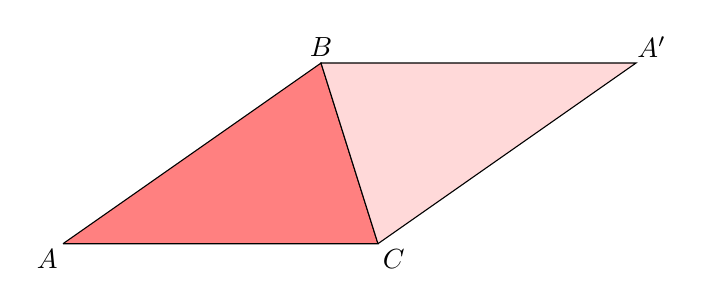
\begin{tikzpicture}
            \draw[fill=red!50] (0, 0) to (4, 0) to (3.27660817716, 2.2943057454 ) to (0,0);
        	\draw[fill=red!15] (4, 0) to (3.27660817716, 2.2943057454 ) to (7.27660817716, 2.2943057454 ) to (4,0);
            \node[] at (-0.2, -0.2) {$A$};
            \node[] at (3.27660817716, 2.4943057454) {$B$};
            \node[] at (4.2, -0.2) {$C$}; 
            \node[] at (7.47660817716, 2.4943057454) {$A'$};
        \end{tikzpicture}
        \captionof{figure}{Square of side length $a+b$. }
        \label{fig:pythag1}
    \end{center}
\end{proof}


\subsubsection*{Disproving Existential Statements: Non-existence Proofs}

When a theorem claims that something does not exist, it is generally a good idea to try a contrapositive or a contradiction proof. This is since `does not exist' is already a \emph{negative} statement. A contradiction or contrapositive proof of a theorem $\timplies PQ$ already involves the negated statement $\neg Q$. If $Q$ states that something does not exist, then $\neg Q$ states that it does, which often gives you something to play with! To see this in action, consider the following result.

\begin{thm}
The equation $x^{17}+12x^3+13x+3=0$ has no positive (real number) solutions.
\end{thm}

\noindent First we interpret the theorem as an implication: throughout we assume that $x$ is a real number.
\[\text{For all $x$, if $x^{17}+12x^3+13x+3=0$, then $x\leq 0$.}\]
The theorem is now in the form $\forall x (\timplies{P(x)}{Q(x)})$, with:
\[P(x):\quad x^{17}+12x^3+13x+3=0,\qquad\qquad\qquad Q(x):\quad x\le 0.\]
The negation of $Q(x)$ is simply `$x>0$.' To prove the theorem by contradiction, we assume $\exists x \, (P(x) \land \neg Q(x))$, and deduce a contradiction.


\begin{proof}
Assume that a real number $x$ satisfies $x^{17}+12x^3+13x+3=0$, and that $x>0$. Because all terms on the left hand side are positive, we have $x^{17}+12x^3+13x+3>0$. A contradiction.
\end{proof}


\noindent Note how quickly the proof is written: it assumes that any reader is familiar with the underlying logic of a contradiction proof without it needing to be spelled out. The discussion we undertook before writing the proof would be considered scratch work: you shouldn't include it a final write-up.\\

\noindent If you want to extend the above result, and you can recall the Intermediate and Mean Value Theorems from Calculus, you should be able to prove that there is exactly one (necessarily negative!) solution to the above polynomial equation.

% \subsubsection*{The AM-GM inequality}

% Next we give several proofs of a famous inequality relating the arithmetic and geometric means of two or more numbers.

% \begin{thm}\label{thm:amgm}
% If $x,y$ are positive real numbers, then
% \[\frac{x+y}{2}\ge\sqrt{xy}\]
% with equality if and only if $x=y$.
% \end{thm}

% \noindent This is a little tricky to read: we really have two separate theorems:
% \begin{enumerate}
%   \item If $x,y>0$, then $\frac{x+y}{2}\ge\sqrt{xy}$
%   \item If $x,y>0$, then $\frac{x+y}{2}=\sqrt{xy}\iff x=y$
% \end{enumerate}

% \noindent First we give a direct proof: note how the implication signs are stacked to make the argument clearer.

% \begin{proof}[Direct Proof]
% Clearly $(x-y)^2\ge 0$ with equality $\iff x=y$. Now multiply out:
% \begin{align*}
% x^2-2xy+y^2\ge 0&\iff (x^2+2xy+y^2)- 4xy  \ge 0 \\
% &\iff x^2+2xy+y^2\ge 4xy\\
% &\iff (x+y)^2\ge 4xy\\
% &\iff x+y\ge 2\sqrt{xy}\tag*{($\ast$)}\\
% &\iff \frac{x+y}{2}\ge \sqrt{xy}.
% \end{align*}
% The square-root in $(\ast)$ is well-defined because $x+y$ is positive.\footnote{Moreover, the inequality is preserved since the function $f(t)=t^2$ is \emph{increasing} when $t$ is positive.} Moreover, it is clear that the final inequality is an equality if and only if all of them are, which is if and only if $x=y$.
% \end{proof}

% \noindent Observe how the argument for `with equality if and only if $x=y$' depends on all of the implications in the proof being \emph{biconditionals}.

% \noindent The following contradiction proof incorporates exactly the same calculation, but is laid out in a different order. This is not always possible, and you have to take great care when trying it. You will likely agree that the direct proof is easier to follow.

% \begin{nopgbreak}
% \begin{proof}[Contradiction Proof]
% Suppose that $\frac{x+y}{2}<\sqrt{xy}$. Since $x+y\ge 0$, this is if and only if $(x+y)^2<4xy$. Now multiply out and rearrange:
% \begin{align*}
% (x+y)^2<4xy&\iff x^2+2xy+y^2<4xy\\
% &\iff x^2-2xy+y^2<0\\
% &\iff (x-y)^2<0.
% \end{align*}
% Since squares of real numbers are non-negative, this is a contradiction. Thus $\frac{x+y}{2}\ge \sqrt{xy}$.\\
% Now suppose that $\frac{x+y}{2}=\sqrt{xy}$. Following the biconditionals through the above argument, we see that this is if and only if $(x-y)^2=0$, from which we recover $x=y$. Hence result.
% \end{proof}
% \end{nopgbreak}


% \subsubsection*{Optional: The general AM-GM inequality}

% Both the statement and the proof of the general inequality are significantly more difficult. You might be surprised that an argument involving `raising to the $n$th power' doesn't work. Try it and see why\ldots\ It is often the case that a very simple proof exists for a special case of a result, and that attempting to generalize the proof fails. A completely new approach is then required.\\
% Since the general result is harder, we present it at a higher level, leaving out some of the more obvious details. This helps us view the proof as a whole, and makes the logical flow clearer. The only prerequisite is a little calculus, namely the First Derivative Test at the end of the first paragraph.

% \begin{thm}
% If $x_1,\ldots,x_n>0$ then
% \[\frac{x_1+x_2+\cdots+x_n}n\ge\sqrt[n]{x_1x_2\cdots x_n}\]
% with equality if and only if $x_1=\cdots =x_n$.
% \end{thm}

% \begin{proof}
% Consider the function $f(x)=e^{x-1}-x$. Its derivative is $f'(x)=e^{x-1}-1$, which is zero if and only if $x=1$. The sign of the derivative changes from negative to positive at $x=1$, whence this is a local minimum. $f$ has no other critical points and its domain is the whole real line, whence $x=1$ is the location of the \emph{global} minimum of $f$. Since $f(1)=0$, we obtain the inequality
% \[e^{x-1}\ge x\tag*{($\dag$)}\]
% with equality if and only if $x=1$.

% \noindent Now consider the arithmetic mean $\mu=\frac{x_1+x_2+\cdots +x_n}{n}$. Applying ($\dag$) to $x=\frac{x_i}\mu$, we obtain
% \[\frac{x_i}\mu\le\exp\left(\frac{x_i}\mu-1\right),\qquad\text{for each $i=1,2,\ldots,n$.}\tag*{($\ast$)}\]
% Since all the $x_i$ are positive, we may multiply the expressions $(\ast)$ while preserving the inequality:
% \[\frac{x_1}\mu\cdots\frac{x_n}\mu\le\exp\left(\frac{x_1}{\mu}-1+\cdots+\frac{x_n}{\mu}-1\right)=\exp(n-n)=1.\]
% It follows that $\mu^n\ge x_1\cdots x_n$, from which the result, $\mu\ge\sqrt[n]{x_1\cdots x_n}$, is clear.\\
% Equality is if and only if all the inequalities $(\ast)$ are equalities, which is if and only if $x_i=\mu$ for all $i=1,\ldots,n$. That is, all the $x_i$ are equal.
% \end{proof}

% \noindent Given that the theorem and proof are both more difficult than the $n=2$ case, there are a few things you should do to help convince yourself of their legitimacy.
% \begin{enumerate}\setlength{\itemsep}{0pt}
%   \item Write down some examples. E.g. if $x_1=20,x_2=27,x_3=50$, the inequality reads
%   \[\frac{97}3\ge\sqrt[3]{20\cdot 27\cdot 50}=30.\]
%   \item Observe that Theorem \ref{thm:amgm} is a special case.
%   \item Work through the proof, inserting comments and extra calculations until you are convinced that the argument is correct. For example, the calculation $\frac{x_1+\cdots+x_n}{\mu}=\frac{\mu n}\mu=n$ was omitted from the final displayed calculation: anyone with the prerequisite knowledge to read the rest of the proof should easily be able to supply this.
% \end{enumerate}

% \noindent It is perfectly reasonable to ask how you would know to try such a proof. The answer is that you wouldn't. You should appreciate that a proof like this is a distillation of thousands of attempts and improvements, perhaps over many years. No-one came up with this argument as a first attempt!


\subsubsection*{Combining and Subdividing Theorems}

Sometimes it is useful to break a proof into pieces, akin to viewing a computer program as a collection of subroutines that you combine for some greater purpose. Usually the intention is to make the proof of a difficult result more readable, but you may also wish to emphasize the importance of certain aspects of your work. Mathematics does this by using \emph{lemmas} and \emph{corollaries.}

\begin{itemize}\setlength{\itemsep}{0pt}
  \item[]\emph{Lemma:} a theorem whose importance you want to downplay. Often the result is individually unimportant, but becomes more useful when referenced in the proof of a larger theorem.
  \item[]\emph{Corollary:} a theorem which follows quickly from another result. Corollaries can be used to draw attention to a particular aspect or a special case of a theorem.
\end{itemize}

\noindent In many mathematical papers the word \emph{theorem} is reserved only for the most important results, everything else being presented as a lemma or corollary. The choice of what to call a result is entirely one of presentation. If you want your paper to be more readable, or to highlight what you think is important, then lemmas and corollaries are your friends!\pagebreak[2]

\noindent Here is a famous example of a lemma at work.

\begin{lemm}\label{lemm:root2prep}
Suppose that $n\in\Z$. Then $n^2$ is even $\iff n$ is even.
\end{lemm}

\noindent Prove this yourself: the ($\Rightarrow$) direction is easiest using the contrapositive method, while the ($\Leftarrow$) direction works well directly.

\begin{thm}\label{thm:root2}
$\sqrt 2$ is irrational.
\end{thm}

% \noindent This is tricky for a few reasons. The theorem does not appear to be of the form $\timplies P{Q,}$ but in fact it is. Consider:
% \begin{itemize}\setlength{\itemsep}{0pt}
%   \item[]\itemstart{$Q$.} $\sqrt 2$ is irrational.
%   \item[]\itemstart{$P$.} Everything you already know in mathematics!
% \end{itemize}
% Of course $P$ is entirely unhelpful; how can we start a direct proof when we don't know what to choose from the whole universe of mathematics? A contrapositive proof might also be difficult: $\neg Q$ straightforwardly states that $\sqrt 2$ is rational, but $\neg P$ is the cryptic statement, `something we know to be true is actually false.' But what is the \emph{something}?\\
% Rather than worry about all this, we instead present a proof by contradiction.

\noindent This is tricky for a few reasons. The theorem does not appear to be of the form $\timplies P{Q,}$, nor does it seem to be any of the forms covered in this section. However, let us look a little closer at what is being claimed. Remember \emph{irrational} simply means \emph{not rational}, i.e., not of the form $m,n$ for $m \in \Z$ and $n \in \N$. Thus saying that $\sqrt{2}$ is irrational is equivalent to saying that there are no $m,n \in \N$ such that $\sqrt{2} = \frac{m}{n}$. Phrased like this, we can see that the theorem statement is really a non-existence statement, and so it makes sense to try a proof by contradiction.

\begin{proof}[Proof.\hspace{-27pt}]
\begin{itemize}\setlength{\itemsep}{-2pt}
  \item[] Suppose that $\sqrt 2=\frac mn$ for some $m,n\in\N$. Without loss of generality, we may assume that $m,n$ have no common factors.
  \item[] Then $m^2=2n^2$ which says that $m^2$ is even.
  \item[] By Lemma \ref{lemm:root2prep} we have that $m$ is even.
  \item[] Thus $m=2k$ for some $k\in\Z$.
	\item[] But now, $n^2=2k^2$, from which (Lemma \ref{lemm:root2prep} again) we see that $n$ is even.
	\item[] Now $m$ and $n$ have a common factor of 2. This is a contradiction.\qedhere
\end{itemize}
\end{proof}

\noindent First observe how Lemma \ref{lemm:root2prep} was used to make the proof easier to read.
Without the lemma, the essential shape of the proof would have been less clear.\\
Now try to make sense of the proof. In the first line we invoke the definition of \emph{rational,} being the \emph{ratio} of two integers. The main challenge comes immediately afterwards. Once we assume that $\sqrt 2=\frac mn$, we can immediately insist that $m,n$ have no common factors. Indeed this is no significant restriction \emph{once we assume that $m,n$ exist,} that is \emph{once we assume that $\sqrt 2$ is rational.} It is important to realize that the `no common factors' assumption is \emph{not} the assumption being contradicted. Because of this subtlety, we include the phrase `without loss of generality' so that the reader is forced to think carefully, and does not jump to the wrong conclusion.\\
It might seem difficult to completely understand, but if we hadn't made the observation, our calculation could have continued forever, telling us nothing!
\[m^2=2n^2\implies n^2=2k^2\implies k^2=2l^2\implies\cdots\]
If you find this approach difficult, you may prefer an alternative proof given in the exercises.


\subsubsection*{Non-constructive Proofs}
% Let's augment our discussion of proofs with what we've learned about quantifiers.
% Consider the following statement: ``there are irrational numbers $a$ and $b$ such that $a^b$ is a rational number.''
% We can formulate this sentence using quantifiers:
% \[
%     \exists a,b\in \R \setminus \Q \left( a^b \in \Q\right).
% \]
% Here, $A\setminus B$ is the \emph{set difference}, which consists of all the elements of $A$ that are \emph{not} in $B$, so $\R\setminus \Q$ is the set of irrational (real) numbers.

% If this proposition is true, then we can prove it by finding specific irrational $a$ and $b$ and demonstrating that $a^b$ is rational.
% Since this proposition is indeed true, we restate it as a theorem and provide a proof.
We saw earlier that we usually prove an existential statement by coming up with an explicit object and showing that it has the desired properties.
Here is an example that shows that this can be a bit subtle.
\begin{thm}
    There are irrational numbers $a$ and $b$ such that $a^b$ is a rational number.
\end{thm}
\begin{proof}
    By Theorem \ref{thm:root2}, we know that $\sqrt{2}$ is irrational.
    Consider the number $(\sqrt{2})^{\sqrt 2}$.
    There are two possibilities.
    If $(\sqrt{2})^{\sqrt 2}$ is rational, then we can take $a = b = \sqrt 2$ in the theorem statement and we're done.
    On the other hand, if $(\sqrt{2})^{\sqrt 2}$ is irrational, then we have
    \[
        \left(\sqrt{2}^{\sqrt 2}\right)^{\sqrt 2} = (\sqrt 2)^{\sqrt 2\cdot \sqrt 2} = (\sqrt 2)^2 = 2.
    \]
    In this case, we can take $a = (\sqrt 2)^{\sqrt 2}$ and $b = \sqrt 2$ in the theorem statement.
    In both cases we have found irrational numbers $a$ and $b$ where $a^b$ is rational.
\end{proof}

The critical, and perhaps unsatisfying, part of this proof is that we have \emph{not} said whether or not $(\sqrt 2)^{\sqrt 2}$ is rational.
We then say that this proof is \emph{non-constructive} since it does not actually contain explicit (and unconditional) irrational $a$ and $b$ with $a^b$ rational.
Instead, we have shown that the theorem is true \emph{whether or not} $(\sqrt 2)^{\sqrt 2}$ is rational.
\subsubsection*{Prime Numbers}

Here is another famous result, dating back at least to the Ancient Greeks (Euclid's \emph{Elements}, Proposition IX.20). As ever, we need a solid definition before we try to prove anything.

\begin{defn}\label{defn:irreducible}
An integer $\ge 2$ is \emph{prime} if the only positive integers it is divisible by are itself and 1.
\end{defn}

\noindent The first few primes are $2,3,5,7,11,13,17,19,\ldots$ It follows\footnote{This is not completely obvious: we will prove it much later in Theorem \ref{thm:fundarith}.} from the definition that all positive integers $\ge 2$ are either primes or \emph{composites} (products of primes). In particular, every integer $\ge 2$ is divisible by at least one prime. We may now state Euclid's result.

\begin{thm}
There are infinitely many prime numbers.
\end{thm}

\begin{proof}
We prove by contradiction. Assume there are exactly $n$ prime numbers $\lst p n$ and consider the integer
\[\Pi:=p_1\cdots p_n+1.\]
Certainly $\Pi$ is divisible by some prime: since we are assuming that the list $\lst pn$ contains \emph{all} the primes, $\Pi$ must be divisible by some prime $p_i$ in the list. However, the product $p_1\cdots p_n$ is clearly divisible by $p_i$, whence so is the difference\footnote{Is this obvious? Can you prove it?!}
\[\Pi-p_1\cdots p_n=1.\]
We conclude that 1 is divisible by the prime $p_i$, contradicting\footnote{Euclid's original argument was not strictly by contradiction. Instead he asserted that, given any list of primes $p_1,\ldots,p_n$, the number $\Pi$ must be divisible by a new prime not in his list.} the fact that $p_i\ge 2$.
\end{proof}





% \paragraph{Self-test Questions}

% \begin{enumerate}
%   \item Consider a theorem $P\implies Q$. We call $P$ the \underline{\phantom{hypothesis}\qquad\qquad} and $Q$ the \underline{\phantom{conclusion}\qquad\qquad}
%   \item In a \emph{proof by contrapositive,} we assume that \underline{\phantom{$Q$ is false}\qquad\qquad} and deduce that \underline{\phantom{$P$ is false}\qquad\qquad}
%   \item A \emph{proof by contradiction} begins by assuming that \underline{\phantom{$P$ is true and $Q$ is false}\qquad\qquad}
%   %\item Propositions are joined by \underline{\phantom{connectives}\qquad\qquad}
%   \item Explain in a sentence or two what is meant by \emph{without loss of generality,} and how the phrase is used.
% \end{enumerate}

\subsection*{Reading Quiz}

\begin{enumerate}
  %\item Consider a theorem $P\implies Q$. We call $P$ the \underline{\phantom{hypothesis}\qquad\qquad} and $Q$ the \underline{\phantom{conclusion}\qquad\qquad}
  
  \item When proving a non-existence statement, i.e., proving that something \emph{does not} exist, proof by contradiction is often useful because \rule{5cm}{0.15mm}.
  
  \begin{enumerate}
      \item contradiction is more powerful than a direct proof.
      \item direct and contrapositive proofs are too complicated.
      \item it allows one to assume such an object exists, hence giving an object that can be manipulated.
      \item it allows one to assume such an object does not exist, which is exactly what the problem is asking for.
  \end{enumerate}
  
  \item True or False: When proving a universal statement like $\forall x\, P(x)$, it suffices to give an explicit example of an $x$ for which $P(x)$ holds.

  \item True or False: When proving an existential statement like $\exists x\, P(x)$, it suffices to give an explicit example of an $x$ for which $P(x)$ holds.

  \item In the proof that $\sqrt{2}$ is irrational, we started by assuming that $\sqrt{2} = \frac{m}{n}$ for integers $m$ and $n$ \emph{with no common factors}. Why is this justified?

  \begin{enumerate}
      \item Because no pair of two integers ever has a common factor.
      \item Because any rational number $\frac{m}{n}$ can be seen, by canceling the common factors of $m$ and $n$, to be equal to a rational $\frac{m'}{n'}$ where $m'$ and $n'$ have no common factors.
      \item It is not justified, we have lost generality by making this assumption.
      \item Because $\sqrt{2}$ is irrational.
  \end{enumerate}
  
  % \item Which of the following would serve as a counterexample to the statement ``any continuous function defined on the open interval $(0,1)$ has a maximum value''?
  
  % \begin{enumerate}
  %     \item There is no counterexample because the statement is true.
  %     \item The function $f(x) = \sin x$.
  %     \item The function $f(x) = 1/x$.
  %     \item The function $f(x)$ where $f(0) = 1$ and $f(x) = 0$ if $x \neq 1$.
  % \end{enumerate}
  
  %\item Propositions are joined by \underline{\phantom{connectives}\qquad\qquad}
  %\item Explain in a sentence or two what is meant by \emph{without loss of generality,} and how the phrase is used.
\end{enumerate}

\subsection*{Practice Problems}

\begin{enumerate}\renewcommand{\labelenumi}{\thesubsection.\theenumi} 
  \item Prove or disprove the following conjectures:\prelistskip
	\begin{enumerate}
	  \item The sum of any 3 consecutive integers is divisible by 3.
	  \item The sum of any 4 consecutive integers is divisible by 4.
	  \item The product of any 3 consecutive integers is divisible by 6.
	\end{enumerate}
	
	  
  \href{https://youtu.be/R5zpsZoR16w}{Video Solution}
	
    \item Critique the following proof.
    If the proof adequately demonstrates why the statement is true, explain why.
    Otherwise, identify any errors and explain how to correct them.
    \begin{thm}
        If $x$ is a positive real number, then $x > 1$ if and only if $1/x < 1$.
    \end{thm}
    \begin{proof}
        Suppose $1/x < 1$.
        Since $x$ is positive, multiplying both sides of this inequality by $x$ does not reverse the inequality and we obtain $1 < x$.
    \end{proof}
	% (From previous exercises)
	
	\href{https://youtu.be/R_W3wwJRlmQ}{Video Solution}
	
\end{enumerate}

\subsection*{Exercises}

\begin{enumerate}\renewcommand{\labelenumi}{\thesubsection.\theenumi}


  \item Prove or disprove the following conjectures.\prelistskip
	\begin{enumerate}
	  \item There is an even integer which can be expressed as the sum of three even integers.
	  \item Every even integer can be expressed as the sum of three even integers. 
	  \item There is an odd integer which can be expressed as the sum of two odd integers.
	  \item Every odd integer can be expressed as the sum of three odd integers.
		\item[]\emph{To get a feel about whether a claim is true or false, try out some examples. If you believe a claim is false, provide a specific counterexample. If you believe a claim is true, give a formal proof.}
\end{enumerate}

	\item Let $P$ be the proposition: `Every positive integer is divisible by thirteen.'\prelistskip
    \begin{enumerate}
      \item Write $P$ using quantifiers.
      \item What is the negation of $P$?
      \item Is $P$ true or false? Prove your assertion.
    \end{enumerate}

%   \item Prove or disprove the following conjectures:\prelistskip
% 	\begin{enumerate}
% 	  \item The sum of any 3 consecutive integers is divisible by 3.
% 	  \item The sum of any 4 consecutive integers is divisible by 4.
% 	  \item The product of any 3 consecutive integers is divisible by 6.
% 	\end{enumerate}

	\item \begin{enumerate} \item Prove or disprove: There exist integers $m$ and $n$ such that $2m-3n=15$. 
	\item Prove or disprove: There exist integers $m$ and $n$ such that $6m-3n=11$. 
  \end{enumerate}

  \item Prove or disprove: There exist a line $L$ in $\R^2$ such that, for all points $A, B \in \R^2$, we have $A, B$ lie on $L$. 

  
	\item Prove that between any two distinct rational numbers there exists another rational number.\label{ex:rationalsdenseinthemselves}
	
	  \item Consider the statement:
  \begin{center}
      For any non-zero rational number $r$ and any irrational number $t$, $rt$ is irrational.
  \end{center}
  \begin{enumerate}
      \item Translate this statement into logic using quantifiers and propositional functions.
      \item Prove the statement.
  \end{enumerate}

	\item Let $p$ be an odd integer. Prove that $x^2-x-p=0$ has no \emph{integer} solutions.
   
	\item Prove: For every positive integer $n$, $n^2+n+3$ is an odd integer greater than or equal to 5.\\
	\emph{There are two claims here: $n^2+n+3$ is odd, and $n^2+n+3\ge 5$.}
	  
	\item In this question, you should use the following definition of the rational numbers.
		\begin{defn*}
  	A real number $x$ is \emph{rational} if it may be written in the form $x=\frac pq$ where $p$ is an integer and $q$ is a positive integer. $x$ is \emph{irrational} if it is not rational.
  	\end{defn*}
  	Prove or disprove the following conjectures.
  	\begin{conj*}[1]
			If $x$ and $y$ are real numbers such that $3x+5y$ is irrational, then at least one of $x$ and $y$ is irrational.
		\end{conj*}
  	\begin{conj*}[2]
			If $x$ and $y$ are rational numbers, then $3x+4xy+2y$ is rational.
		\end{conj*}
  	\begin{conj*}[3]
			If $x$ and $y$ are irrational numbers, then $3x+4xy+2y$ is irrational.
		\end{conj*}
	
% 	\item Let $x$ and $y$ be integers. Prove: For $x^2+y^2$ to be even, it is necessary that $x$ and $y$ have the same parity (i.e. both even or both odd).
	
  \item \emph{(Snake-like integers)} Let's say that an integer $y$ is \textit{Snake-like} if and only if there is some integer $k$ such that $y=(6k)^2+9$.
	\begin{enumerate}
	  \item Give three examples and three non-examples of Snake-like integers. 
	  \item Given $y\in\Z$, compute the negation of the statement, `$y$ is Snake-like.'
	  \item Show that every Snake-like integer is a multiple of $9$.
	  \item Show that the statements, `$n$ is Snake-like,' and, `$n$ is a multiple of nine,' are not equivalent.
	\end{enumerate}
	
    \item Prove that it is never the case that $x^2 = 2y^2$ for integers $x$ and $y$.
  
  \item Here is an alternative argument that $\sqrt 2$ is irrational. Suppose that $\sqrt 2=\frac mn$ where $m,n\in\N$. This time we don't assume that $m,n$ have no common factors.
  \begin{enumerate}
    \item $m,n$ satisfy the equation $m^2=2n^2$. Prove that there exist positive integers $m_1,n_1$ which satisfy the following three conditions:
    \[m_1^2=2n_1^2,\qquad\qquad m_1<m,\qquad\qquad n_1<n.\] 
    \item Show that there exist two sequences of decreasing positive integers $m>m_1>m_2>\cdots$ and $n>n_1>n_2>\cdots$ which satisfy $m_i^2=2n_i^2$ for all $i\in\N$.
    \item Is it possible to have an infinite sequence of decreasing \emph{positive} integers? Why not? Show that we obtain a contradiction and thus conclude that $\sqrt 2\not\in\Q$.
	\end{enumerate}
	This is an example of the \emph{method of infinite descent,} which is very important in number theory. 
	
		\item The real numbers have the \emph{Archimedean property}, that is, for any positive real numbers $x$ and $y$, there exists a positive integer $n$ such that $nx > y$. Use this fact to show that there do not exist any positive real numbers which are less than $1/n$ for all positive integers $n$. 
  
    \item Consider the following proof of the fact that every real number is less than some positive integer:
  \begin{proof}
      Consider a real number $x$. For example, $x = 19.7$. Then $x < 20$ and $20$ is a positive integer. 
  \end{proof}
  What is wrong with this proof? Give a correct proof. [Hint: use the previous exercise.]
	
	\item Here is an extension of question \ref{ex:rationalsdenseinthemselves}. Let $\lceil x\rceil$, the \emph{ceiling} of $x$, denote the smallest integer greater than or equal to $x$. E.g.\ $\lceil 3.2\rceil=4$, $\lceil 7\rceil=7$ and $\lceil -8.4\rceil=-8$.
	\begin{enumerate}
  	\item Suppose that $x$ and $y$ are real numbers with $x<y$. Use the ceiling function to show that there exists a positive integer $n$ for which $n(y-x)>1$.
  	\item Prove or disprove: $\forall x,y\in\R$ with $x<y$, $\exists m,n\in\Z$ for which $nx<m<ny$.
  	\item Use parts (a) and (b) to prove that between any two real numbers there exists a rational number.
  	\item (Hard) Is it true that between any two real numbers there exists an \emph{irrational} number? If so, prove it.
	\end{enumerate}
	
	\item Suppose that $x,y,z$ are real numbers such that $x + y + z = 1$. Prove
    \[  
        (1 - x)(1 - y)(1 - z) \geq 8 xyz.
    \]
    [Hint: find a way to apply the AM-GM inequality.]
    
    % \item Use the general AM-GM inequality to establish
    % \[
    %     n! \leq \left(\frac{n + 1}{2}\right)^n.
    % \]
	
  \item You are given the following facts.
  \begin{enumerate}
    \item All polynomials are continuous.
    \item (Intermediate Value Theorem) If $f$ is continuous on $[a,b]$ and $L$ lies between $f(a)$ and $f(b)$, then $f(x)=L$ for some $x\in(a,b)$.
    \item If $f'(x)>0$ on an interval, then $f$ is an increasing function.
	\end{enumerate}
	Use these facts to give a formal proof that $x^{17}+12x^3+13x+3=0$ has \emph{exactly one solution} $x$, and that $x$ lies in the interval $(-1,0)$.
	
		\item (Hard) This question uses Definition \ref{defn:cont}.
		\begin{enumerate}
	  \item Prove, directly from the definition, that $f(x)=x^2$ is continuous at $x=0$. \emph{If you are given $\epsilon>0$, what should $\delta$ be?}
	  \item Prove that $g(x)=\begin{cases}
	  1+x&\text{if }x\ge 0,\\
	  x&\text{if }x<0,
	  \end{cases}$\quad 
	  is discontinuous at $x=0$.
	  \item (Very hard) Let $h(x)=\begin{cases}
	  x&\text{if $x$ is rational,}\\
	  0&\text{if $x$ is irrational.}
	  \end{cases}$\quad Prove that $f$ is continuous \emph{only} at $x=0$.
	  \end{enumerate}\goodbreak
	
	\item (Hard) In this question we prove Rolle's Theorem from calculus:
	\begin{quote}
	Suppose $f$ is continuous on $[a,b]$, differentiable on $(a,b)$, and $f(a)=f(b)=0$, then $\exists c\in(a,b)$ such that $f'(c)=0$.
	\end{quote}
	 As you work through the question, think about where the hypotheses are used and why we need them.
    \begin{enumerate}
      \item Recall the Extreme Value Theorem. The function $f$ is continuous on $[a,b]$, so $f$ is bounded and attains its bounds. Otherwise said,
      \[\exists m,M\in[a,b]\text{ such that } \forall x\in[a,b]\text{ we have }f(m)\le f(x)\le f(M).\]
      Suppose that $f(m)=f(M)$. Why is the conclusion of Rolle's Theorem obvious in this case?
      \item Now suppose that $f(m)\neq f(M)$. Argue that \emph{at least one} of the following cases holds:
      \[f(M)>0\quad\text{or}\quad f(m)<0.\]
      \item Without loss of generality, we may assume that $f(M)>0$. By considering the function $-f$, explain why.
      \item Assume $f(M)>0$. Then $M\neq a$ and $M\neq b$. Consider the difference quotient,
      \[\frac{f(M+h)-f(M)}h.\]
      Show that if $0<\nm h<\min\{M-a,b-M\}$ then the difference quotient is well-defined (exists and makes sense).
      \item Suppose that $0<h<b-M$. Show that
      \[\frac{f(M+h)-f(M)}h\le 0.\]
      How do we know that $L^+:={\displaystyle\lim_{h\to 0^+}}\frac{f(M+h)-f(M)}h$ exists? What can you conclude about $L^+$?
      \item Repeat part (d) for $L^-:={\displaystyle\lim_{h\to 0^-}}\frac{f(M+h)-f(M)}h$.
      \item Conclude that $L^+=L^-=0$. Why have we completed the proof?
    \end{enumerate}
	
\end{enumerate}


\newpage











